%
%Не забыть:
%--------------------------------------
%Вставить колонтитулы, поменять название на титульнике



%--------------------------------------

\documentclass[a4paper, 12pt]{article} 

%--------------------------------------
%Russian-specific packages
%--------------------------------------
%\usepackage[warn]{mathtext}
\usepackage[T2A]{fontenc}
\usepackage[utf8]{inputenc}
\usepackage[english,russian]{babel}
\usepackage[intlimits]{amsmath}
\usepackage{esint}
%--------------------------------------
%Hyphenation rules
%--------------------------------------
\usepackage{hyphenat}
\hyphenation{ма-те-ма-ти-ка вос-ста-нав-ли-вать}
%--------------------------------------
%Packages
%--------------------------------------
\usepackage{amsmath}
\usepackage{amssymb}
\usepackage{amsfonts}
\usepackage{amsthm}
\usepackage{latexsym}
\usepackage{mathtools}
\usepackage{etoolbox}%Булевые операторы
\usepackage{extsizes}%Выставление произвольного шрифта в \documentclass
\usepackage{geometry}%Разметка листа
\usepackage{indentfirst}
\usepackage{wrapfig}%Создание обтекаемых текстом объектов
\usepackage{fancyhdr}%Создание колонтитулов
\usepackage{setspace}%Настройка интерлиньяжа
\usepackage{lastpage}%Вывод номера последней страницы в документе, \lastpage
\usepackage{soul}%Изменение параметров начертания
\usepackage{hyperref}%Две строчки с настройкой гиперссылок внутри получаеммого
\usepackage[usenames,dvipsnames,svgnames,table,rgb]{xcolor}% pdf-документа
\usepackage{multicol}%Позволяет писать текст в несколько колонок
\usepackage{cite}%Работа с библиографией
\usepackage{subfigure}% Человеческая вставка нескольких картинок
\usepackage{mhchem}
\usepackage{authblk}
\usepackage{mathabx}
\usepackage{tikz}%Рисование рисунков
\usetikzlibrary{circuits} % подключаем библиотеки, содержащие
\usetikzlibrary{circuits.ee} % УГО для схем
\usetikzlibrary{circuits.ee.IEC}
\usetikzlibrary{arrows} % подключаем библиотеки со стрелками
\usetikzlibrary{patterns} % и со штриховкой
\usepackage{float}% Возможность ставить H в положениях картинки
% Для картинок Моти
\usepackage{misccorr}
\usepackage{lscape}
\usepackage{cmap}
\usepackage{bm}
\newtheorem{definition}{Определение}



\usepackage{graphicx,xcolor}
\graphicspath{{Pictures/}}
\DeclareGraphicsExtensions{.pdf,.png,.jpg,.jpeg}

%----------------------------------------
%Список окружений
%----------------------------------------
\newenvironment {theor}[2]
{\smallskip \par \textbf{#1.} \textit{#2}  \par $\blacktriangleleft$}
{\flushright{$\blacktriangleright$} \medskip \par} %лемма/теорема с доказательством
\newenvironment {proofn}
{\par $\blacktriangleleft$}
{$\blacktriangleright$ \par} %доказательство
%----------------------------------------
%Список команд
%----------------------------------------
\newcommand{\grad}
{\mathop{\mathrm{grad}}\nolimits\,} %градиент

\newcommand{\diver}
{\mathop{\mathrm{div}}\nolimits\,} %дивергенция

\newcommand{\rot}
{\ensuremath{\mathrm{rot}}\,}

\newcommand{\Def}[1]
{\underline{\textbf{#1}}} %определение

\newcommand{\RN}[1]
{\MakeUppercase{\romannumeral #1}} %римские цифры

\newcommand {\theornp}[2]
{\textbf{#1.} \textit{ #2} \par} %Написание леммы/теоремы без доказательства

\newcommand{\qrq}
{\ensuremath{\quad \Rightarrow \quad}} %Человеческий знак следствия

\newcommand{\const}{\text{const}} % Написание const в формулах

\newcommand{\qlrq}
{\ensuremath{\quad \Leftrightarrow \quad}} %Человеческий знак равносильности

\renewcommand{\phi}{\varphi} %Нормальный знак фи

\renewcommand{\epsilon}{\varepsilon}

\newcommand{\me}
{\ensuremath{\mathbb{E}}}

\newcommand{\md}
{\ensuremath{\mathbb{D}}}




%----------------------------------------
%Разметка листа
%----------------------------------------
\geometry{top = 3cm}
\geometry{bottom = 2cm}
\geometry{left = 1.5cm}
\geometry{right = 1.5cm}
%----------------------------------------
%Колонтитулы
%----------------------------------------
\pagestyle{fancy}%Создание колонтитулов
\fancyhead{}
%\fancyfoot{}
\fancyhead[R]{\textsc{Экзамен. Введение в молекулярную биологию}}%Вставить колонтитул сюда
%----------------------------------------
%Интерлиньяж (расстояния между строчками)
%----------------------------------------
%\onehalfspacing -- интерлиньяж 1.5
%\doublespacing -- интерлиньяж 2
%----------------------------------------
%Настройка гиперссылок
%----------------------------------------
\hypersetup{				% Гиперссылки
	unicode=true,           % русские буквы в раздела PDF
	pdftitle={Заголовок},   % Заголовок
	pdfauthor={Автор},      % Автор
	pdfsubject={Тема},      % Тема
	pdfcreator={Создатель}, % Создатель
	pdfproducer={Производитель}, % Производитель
	pdfkeywords={keyword1} {key2} {key3}, % Ключевые слова
	colorlinks=true,       	% false: ссылки в рамках; true: цветные ссылки
	linkcolor=blue,          % внутренние ссылки
	citecolor=blue,        % на библиографию
	filecolor=magenta,      % на файлы
	urlcolor=red           % на URL
}
%----------------------------------------
%Работа с библиографией (как бич)
%----------------------------------------
\renewcommand{\refname}{Список литературы}%Изменение названия списка литературы для article
%\renewcommand{\bibname}{Список литературы}%Изменение названия списка литературы для book и report
%----------------------------------------
\begin{document}
	\begin{titlepage}
		\begin{center}
			$$$$
			$$$$
			$$$$
			$$$$
			{\Large{НАЦИОНАЛЬНЫЙ ИССЛЕДОВАТЕЛЬСКИЙ УНИВЕРСИТЕТ}}\\
			\vspace{0.1cm}
			{\Large{ВЫСШАЯ ШКОЛА ЭКОНОМИКИ}}\\
			\vspace{0.25cm}
			{\large{Факультет физики}}\\
			\vspace{5.5cm}
			{\Huge\textbf{{Экзамен}}}\\%Общее название
			\vspace{1cm}
			{\LARGE{<<Введение в молекулярную биологию>>}}\\%Точное название
			\vspace{2cm}
			\vfill
			\includegraphics[width = 0.2\textwidth]{HSElogo}\\
			\vfill
			Москва\\
			2021
		\end{center}
	\end{titlepage}
	
	\tableofcontents
	
	\newpage
	
	\section{Химическая и биологическая эволюция. Наследственность, изменчивость и естественный отбор. Основные таксономические группы живых систем. Строение клетки про- и эукариот (сходства и различия). Единство молекулярных механизмов живых систем (примеры). Организация генома живых существ: хромосомы, ДНК пластид и митохондрий, плазмиды.}

\subsection{Химическая эволюция и биологическая эволюция}

\textbf{Химическая эволюция} --- этап, предшествовавший появлению жизни, в ходе которого органические, пребиотические вещества возникали из неорганических молекул под влиянием внешних энергетических и селекционных факторов и в силу развертывания процессов самоорганизации, свойственных всем относительно сложным системам, которыми, бесспорно, являются все углеродосодержащие молекулы.

\medspace

Пребиотический синтез сложных соединений молекул может делиться на три этапа:

\begin{enumerate}
	\item Возникновение простых органических соединений (спиртов, кислот и т.п.) из неорганических;
	
	\item Синтез более сложных органических соединений — <<биомолекул>> — представителей наиболее распространённых классов метаболитов (продукты метаболизма), в том числе и мономеров --- структурных единиц биополимеров (моносахаридов, аминокислот, жирных кислот, нуклеотидов) из простых органических соединений;
	
	\item Возникновение сложных биополимеров (полисахариды, белки, нуклеиновые кислоты) из основных структурных единиц --- мономеров.
\end{enumerate}

\textbf{Биологическая эволюция} --- любое генетическое изменение в популяции, которое происходило в течение нескольких поколений. Изменения должны происходить на генетическом уровне вида и передаваться от одного поколения к другому.

\subsection{Наследственность, изменчивость и естественный отбор}

\textbf{Наследственность} --- способность организмов передавать свои признаки и особенности развития потомству. Благодаря ей живые существа сохраняют в своих потомках характерные черты вида. Наследственность обеспечивается передачей генетической информации. Например, у эукариот материальными единицами наследственности являются гены, локализованные в хромосомах ядра и ДНК органелл.

\textbf{Изменчивость} --- разнообразие признаков среди представителей данного вида, а также свойство потомков приобретать отличия от родительских форм.

Изменчивость бывает нескольких типов. Выделим парочку:

\begin{itemize}
	\item Наследственная (обусловлена возникновением разных типов мутаций и их комбинаций, которые передаются по наследству и впоследствии проявляются у потомства) и ненаследственная (способность организмов с одинаковым генотипом развиваться по-разному в разных условиях окружающей среды);
	
	\item Индивидуальная (различие между отдельными особями) и групповую (различия между группами особей, например, различными популяциями вида, является производной от индивидуальной).
\end{itemize}

\textbf{Естественный отбор} --- основной фактор эволюции, в результате действия которого в популяции увеличивается число особей, обладающих более высокой приспособленностью к условиям среды (наиболее благоприятными признаками), в то время как количество особей с неблагоприятными признаками уменьшается.

\subsection{Основные таксономические группы живых систем}

Таксономическая группа фактически это уровень в биологической систематике, т.е. в дисциплине, которая разрабатывает принципы классификации живых организмов. Таксоны идут по иерархии, представим ее от более глобальных таксонов к менее глобальным (только основные, иначе можно с ума сойти; в скобках --- название на латыни):

\begin{itemize}
	\item Царство (regnum);
	
	\item Тип (phylum) --- у растений вместо него Отдел (divisio);
	
	\item Класс (classis);
	
	\item Отряд (ordo) --- у растений вместо него Порядок (тоже ordo);
	
	\item Семейство (familia);
	
	\item Род (genus);
	
	\item Вид (species) --- группа организмов с общими морфофизиологическими, биохимическими и поведенческими признаками, способная к взаимному скрещиванию, которое даёт в ряду поколений плодовитое потомство, закономерно распространённая в пределах определённого ареала и сходно изменяющаяся под влиянием факторов внешней среды.
\end{itemize}

\subsection{Строение клетки про- и эукариот (сходства и различия)}

\begin{itemize}
	\item Размер клеток у прокариот сильно (в 1000 - 10000 раз) меньше, чем у эукариот;
	
	\item Прокариоты в основном одноклеточные, в то время как эукариоты все же в основном многоклеточные;
	
	\item Эукариоты сильно моложе (почти на 2 млрд лет) чем прокариоты (первые произошли от вторых);
	
	\item У прокариотов клетки в основном просто делятся пополам, в то время как у эукариотов возможны митозы, мейоз или их комбинация, при этом образуется т.н. веретено деления (т.е. динамическая структура, которая образуется в митозе и мейозе для обеспечения отделения хромосом и деления клетки);
	
	\item У прокариотов кольцевая ДНК просто плавает в цитоплазме, она не связана с белками или РНК, а хромосом нет. У эукариотов же ДНК линейная и локализована в ядре, имеются хромосомы, а днк связана с РНК и белком;
	
	\item У прокариот мелкие (70S) рибосомы, эндоплазматического ретикулума (это внутриклеточный органоид эукариотической клетки, который представляет из себя разветвленную систему из окруженных мембраной уплощенных полостей пузырьков и канальцев) нет (различия и по многим другим деталям белкового синтеза, включая чувствительность к антибиотикам; синтез белков у прокариот, например, подавляется антибиотиком стрептомицином). У эукариот же крупные (80S) рибосомы, которые могут быть прикреплены к эндоплазматическому ретикулуму;
	
	\item Органелл у прокариот мало, ни одна из них не имеет оболочки (двойной мембраны). Внутренних мембран почти нет, редко, когда они есть, их ассоциируют с процессами дыхания и фотосинтеза. У эукариот наоборот (органеллы это например ядро, митохондрии, хлоропласты);
	
	\item Клеточные стенки у прокариот жесткие, содержат полисахариды и аминокислоты, основной опорный материал --- муреин (компонент, выполняющий функцию осмотической защиты клетки). У эукариот бывает по-разному: у зеленых растений и грибов стенки жесткие, содержат полисахариды. У растений они в основном из целлюлозы, у грибов из хитина. У животных клеточной стенки нет;
	
	\item У прокариот жгутики простые, нет микротрубочек (белковые внутриклеточные структуры, входящие в состав цитоскилета, которые представляют собой полые цилиндры диаметром 25 нм. Длина может варьироваться), расположены внеклеточно (не окружены плазматической мембраной). У эукариот же жгутики они сложные, окружены плазматической мембраной. Диаметр их раз в 10 больше;
	
	\item Дыхание у прокариот происходит в мезосомах, у цианобактерий --- на цитоплазматических мембранах. У эукариот же аэробное дыхание, которое происходит в митохондриях;
	
	\item У прокариот не бывает хлоропластов, а фотосинтез (если есть) происходит на мембранах, у которых нет специфической упаковки. У эукариот же появляются хлоропласты (если они делают фотосинтез), состоящие из уложенных в особую структуру мембран;
	
	\item Некоторые прокариоты могут фиксировать азот. Эукариоты так не умеют.
	
\end{itemize}


\subsection{Единство молекулярных механизмов живых систем (примеры)}

Хз. Примеры например:

\begin{itemize}
	\item Единый генетический код;
	
	\item Большинство состоят из клеток (кроме вирусов), которые схожи по внутреннему строению.
\end{itemize}

\subsection{Организация генома живых существ: хромосомы, ДНК пластид и митохондрий, плазмиды}

\subsubsection{Хромосомы}

Вытянутые, структурированные совокупности генов, которые несут информацию о наследственности и образованы и конденсированного хроматина (масса генетического материала, состоящая из ДНК и белков, которые конденсируются с образованием хромосом во время деления эукариотических клеток. Хроматин содержится в ядрах клеток). Наборы хромосом соединяются вместе (один от отца, один от матери) и известны как гомологические хромосомы (пары хромосом, одинаковые по длине, положению генов и местоположению центромеров).

\begin{figure}[H]
	\centering
	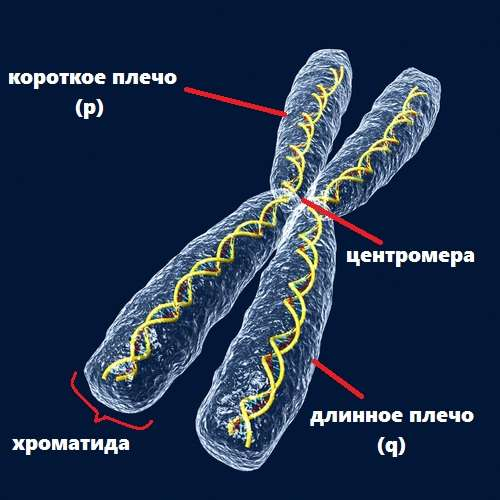
\includegraphics[width=0.7\linewidth]{1_chromosome}
	\caption{Строение хромосомы}
\end{figure}

\subsubsection{ДНК пластид и митохондрий}

И митохондрии, и пластиды --- двухмембранные органоиды эукариотических клеток. Митохондрии встречаются во всех клетках животных и растений, пластиды же характерны для клеток растений, осуществляющих фотосинтетические процессы. Эти органоиды имеют сходный план строения и некоторые общие свойства. Однако по основным метаболическим процессам они существенно отличаются друг от друга.

\begin{itemize}
	\item \textbf{Митохондрии} --- округлые, овальные или палочковидные двухмембранные органоиды диаметром около 0.21 мкм и длиной до 710 мкм. Основная --- функция синтез АТФ.
	
	\item \textbf{Пластиды} --- двухмембранные органоиды, характерные для фотосинтезирующих эукариотных организмов. Различают три основных типа пластид: хлоропласты, хромопласты и лейкопласты. Совокупность пластид в клетке называют пластидомом. Каждый из этих типов при определенных условиях может переходить один в другой. Как и митохондрии, пластиды содержат собственные молекулы ДНК. Поэтому они также способны размножаться независимо от деления клетки.
	
	Пластиды бывают разные:
	
	\begin{itemize}
		\item \textbf{Хлоропласты} --- пластиды, в которых осуществляется фотосинтез.
		
		\item \textbf{Хромопласты} --- окрашенные пластиды. Цвет их обусловлен наличием следующих пигментов: каротина (оранжевожелтый), ликопина (красный) и ксантофилла (желтый). Хромопластов особенно много в клетках лепестков цветков и оболочек плодов.
		
		\item \textbf{Лейкопласты} --- бесцветные пластиды округлой, яйцевидной, веретенообразной формы. Находятся в подземных частях растений, семенах, эпидермисе, сердцевине стебля. Основная функция лейкопластов --- это аккумуляция питательных веществ.
	\end{itemize}
\end{itemize}

Теперь немного про их ДНК. Их характерные черты:

\begin{itemize}
	\item Митохондрии и пластиды имеют собственную специфическую систему синтеза белков (ДНК, РНК, рибосомы). Специфичность этой системы заключается в автономности и резком отличии от таковой в клетке;
	
	\item ДНК митохондрий и пластид представляет собой небольшую циклическую или линейную молекулу, которая отличается от ДНК ядра и по своим характеристикам приближается к ДНК прокариотических клеток. Синтез ДНК митохондрий и пластид не зависит от синтеза ядерной ДНК;
	
	\item В митохондриях и хлоропластах имеются иРНК (информационная), тРНК (транспортная), рРНК (рибосомная). Рибосомы и рРНК этих органоидов резко отличаются от таковых в цитоплазме. В частности рибосомы митохондрий и хлоропластов, в отличие от цитоплазматических рибосом, чувствительны к антибиотику хлорамфениколу, подавляющему синтез белка у прокариотических клеток.
\end{itemize}

\subsubsection{Плазмиды}

Это небольшие молекулы ДНК, физически обособленные от хромосом и способные к автономной репликации. Главным образом плазмиды встречаются у бактерий, а также у некоторых архей и эукариот (грибов и высших растений). Чаще всего плазмиды представляют собой двухцепочечные кольцевые молекулы. Несмотря на способность к размножению, плазмиды, как и вирусы, не рассматриваются в качестве живых организмов. Плазмиды в основном кодируют функции, придающие бактерии преимущество в случае попадания в неблагоприятные условия (например, устойчивость к антибиотикам или, наоборот, синтез антибиотических веществ).

Размеры плазмид варьируют от менее чем 1 тысячи до 400—600 тысяч пар оснований (п. о.). Некоторые плазмиды содержатся в клетке в количестве однойдвух копий, другие — в количестве нескольких десятков. Плазмиды разных классов могут сосуществовать в клетке.

\begin{figure}[H]
	\centering
	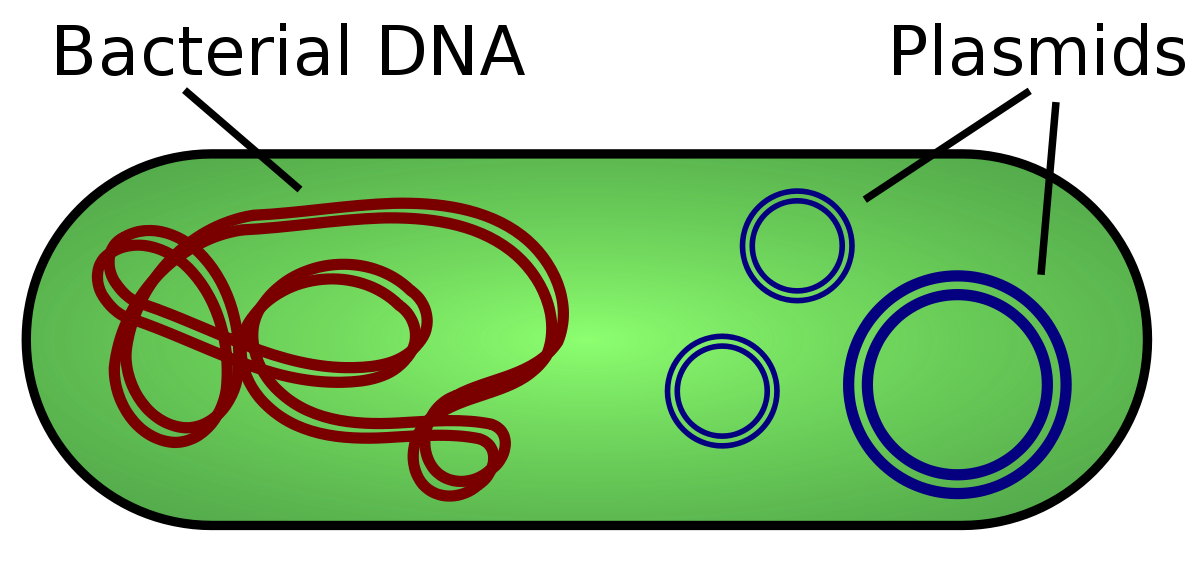
\includegraphics[width=0.7\linewidth]{1_plazmids}
	\caption{Плазмиды и хромосомная ДНК в бактериальной клетке}
\end{figure}
































	
	\newpage
	
	\section{Второй билет. Основные классы биологический молекул, ДНК, генетический код}
Кто хочет подробней открывайте Альбертса с 59ой страницы. Тут только малая часть того что там есть
\subsection{Основыне классы биологический молекул}
\paragraph{Углеводны} Они же сахара. Содержат альдегидную группу $\ce{C=O}$ А так же несколько гидроксильных групп $\ce{O - H}$. Простейшим примером является глюкоза $\ce{C6H12O6}$, которая частный случай моносахарида $\ce{(CH2O)_n}$ где $n$ любое натуральное число. Углеводы могут существовать либо в форме кольца, либо
в виде открытой цепи. К одному кольцо может через атом углерода альдегидной группы присоединиться еще одно кольцо, образуя дисахарид. Например мальтоза (см картинку ниже). Можно образовывать еще большие последовательности, называются полисахаридами.
\begin{figure}[H]
	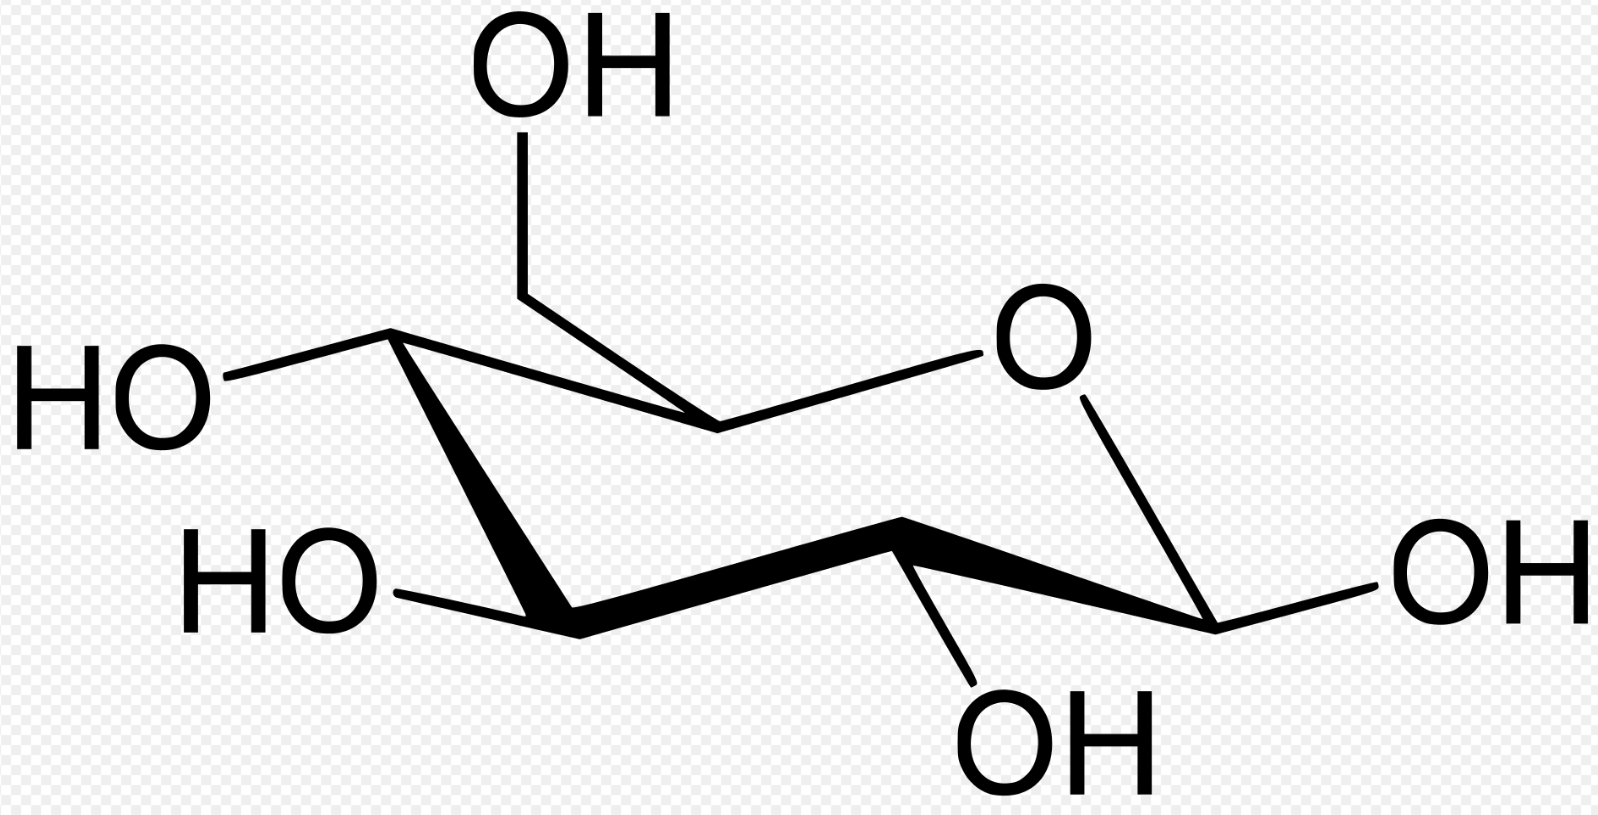
\includegraphics[scale = 0.2]{2glu}\\
	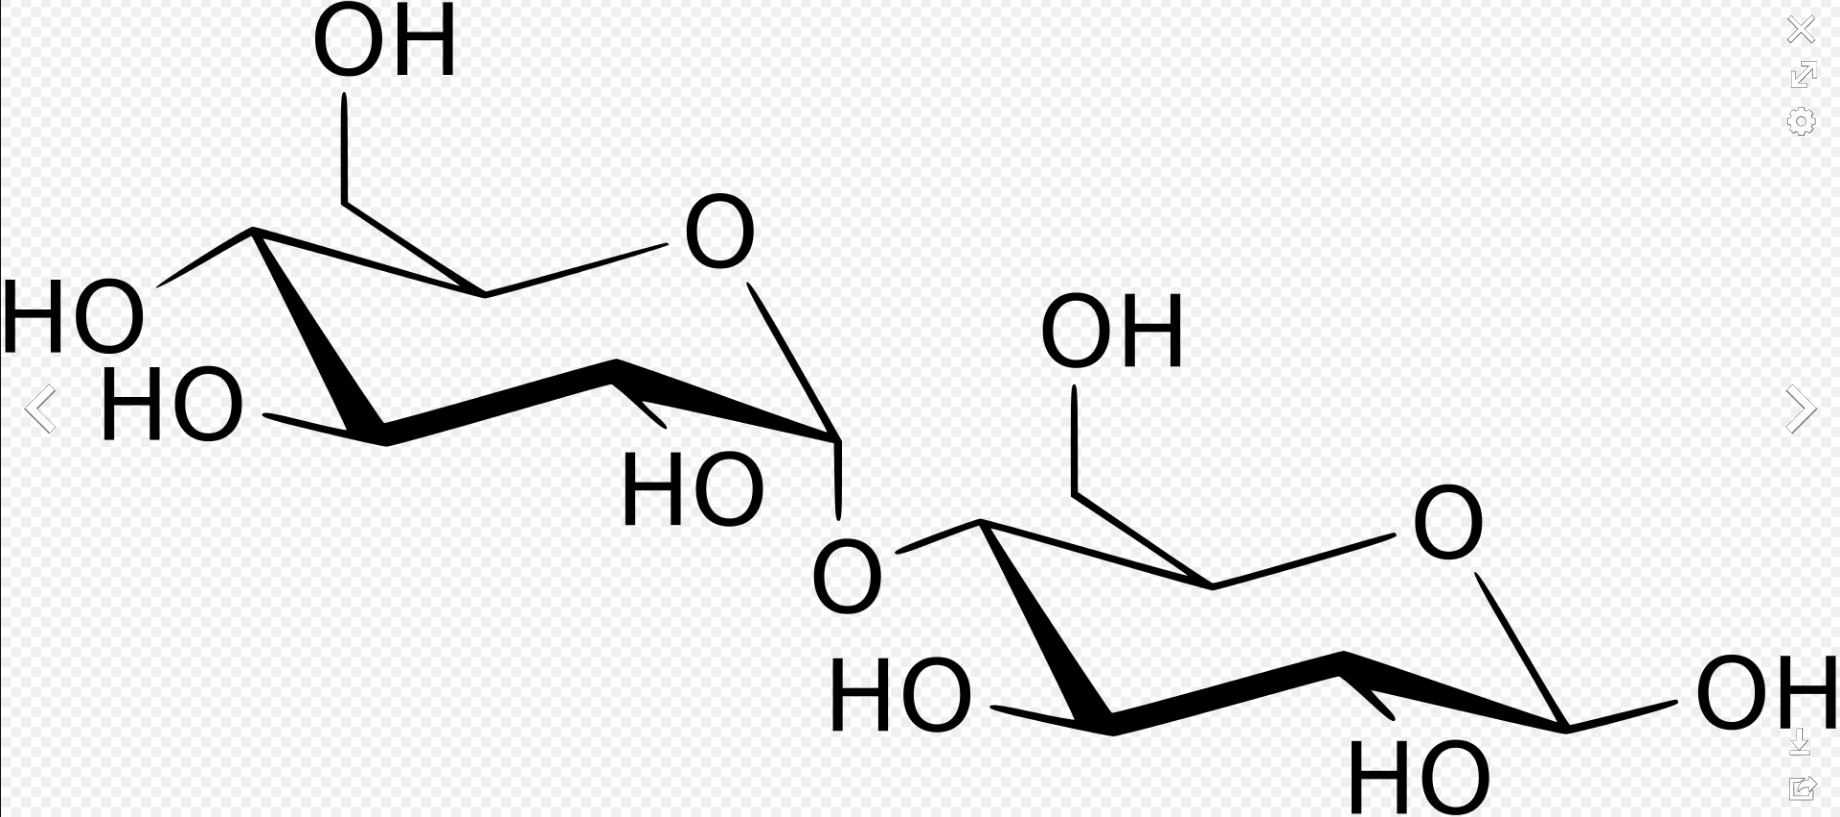
\includegraphics[scale = 0.2]{2mal}
	\caption{Глюкоза и мальтоза}
\end{figure}
Глюкоза служит главным источником энергии во многих клетках. В результате последовательного ряда реакций окисления эта гексоза превращается в различные производные Сахаров с меньшей длиной цепи и в конечном итоге распадается до $\ce{CO2}$ и $\ce{H2O}$. В ходе распада глюкозы высвобождается энергия и генерируется восстановительная способность, без чего невозможно протекание
биосинтетических реакций. Высвобождающаяся энергия и генерируемая восстановительная сила запасаются в форме двух важнейших соединений -
АТР и NADH. Так же из углеводов состоит важный внеклеточный структурный материал (например целлюлоза) 
\paragraph{Липиды} они же жиры. У них обычно имеются две различные части: длинная углеводородная цепь,
которая имеет гидрофобный характер (водонерастворима) и химически мало активна, и карбоксильная группа, ионизирующаяся в растворе, крайне
гидрофильная (водорастворимая) и легко образующая эфиры и амиды.\\
Жирные кислоты являются ценным источником энергии, поскольку их
расщепление сопровождается образованием такого количества АТР, которое в два раза
превышает образование АТР при расщеплении такого же количества (по массе)
глюкозы. Жирные кислоты запасаются в цитоплазме многих клеток в виде капелек
триацилглицеролов (триглицеридов). Молекулы триацилглицеролов состоят из трех
цепей жирных кислот, каждая из которых присоединена к молекуле глицерола  именно так устроены животные жиры, с которыми мы имеем дело в
повседневной жизни.\\
Но самая важная функция жирных кислот - участие в построении клеточных
мембран. Эти тонкие плотные пленки, которыми одеты все клетки и внутриклеточные
органеллы, состоят главным образом из фосфолипидов
\begin{figure}[H]
	\centering
	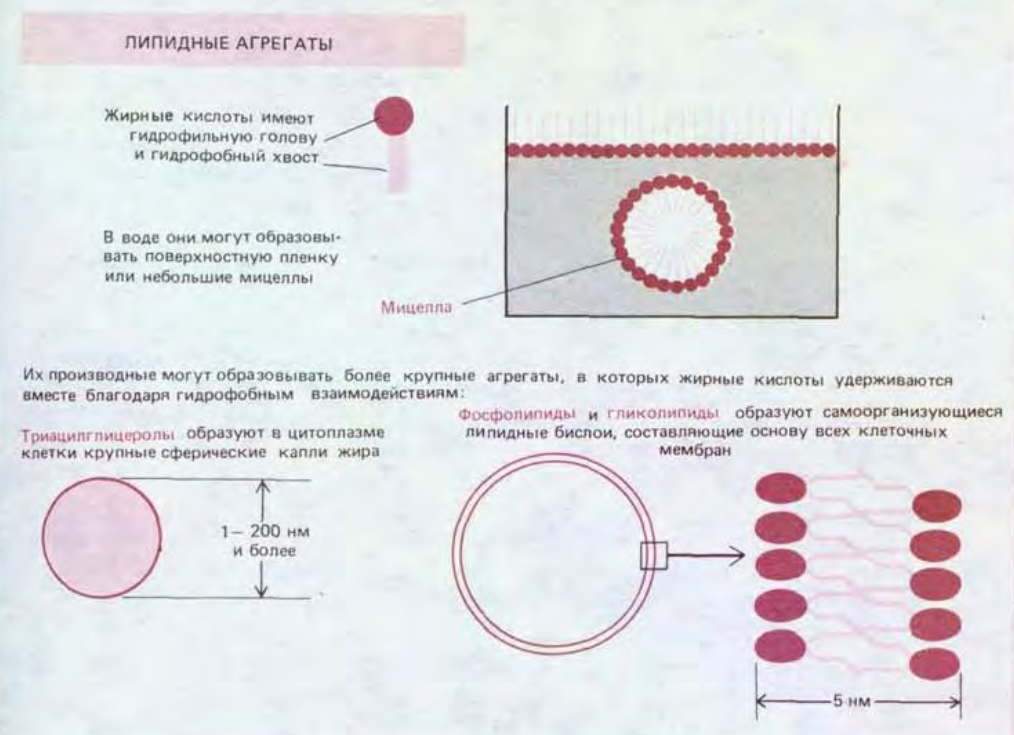
\includegraphics[scale=0.3]{2lipid}
\end{figure}
\paragraph{Аминокислоты} органические вещества которые состоят из аминогруппы и карбоксильной круппы
\begin{figure}[H]
	\centering
	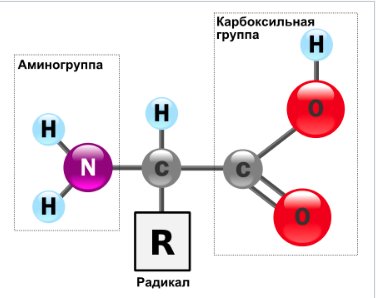
\includegraphics[scale= 0.7]{2amin}
\end{figure}
Аминокислоты служат строительными блоками при синтезе белков
- длинных линейных полимеров аминокислот, соединенных «хвост к голове» при
помощи пептидной связи между карбоксильной группой одной аминокислоты и
аминогруппой другой. В белках встречается обычно 20 аминокислот с
разными радикалами. Одни и те
же 20 аминокислот неоднократно повторяются во всех белках, в том числе в белках
бактериального, животного и растительного происхождения.
\paragraph{Нуклеотиды} Нуклеотиды являются сложными эфирами нуклеозидов и фосфорных кислот.
\begin{figure}[H]
	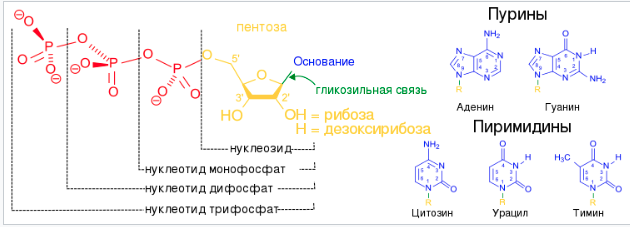
\includegraphics[scale = 0.7]{2nucle}
\end{figure}
Цитозин (С), тимин (Т) и урацил (U)
называются пиримидиновыми основаниями, так как они представляют собой простые производные шестичленного пиримидинового кольца;
гуанин (G) и аденин (А) - пуриновые основания, второе пятичленное кольцо которых сконденсировано с шестичленным циклом\\
Нуклеотиды могут выступать в качестве переносчиков энергии. При этом трифосфатный эфир аденина АТР (рис. 2-9) гораздо чаще, чем
другие нуклеотиды, участвует в переносе энергии между сотнями индивидуальных внутриклеточных реакций. Энергия высвобождающаяся в результате гидролиза АТФ может использоваться в любой другой реакции которая проходит с поглощением энергии.
\begin{figure}[H]
	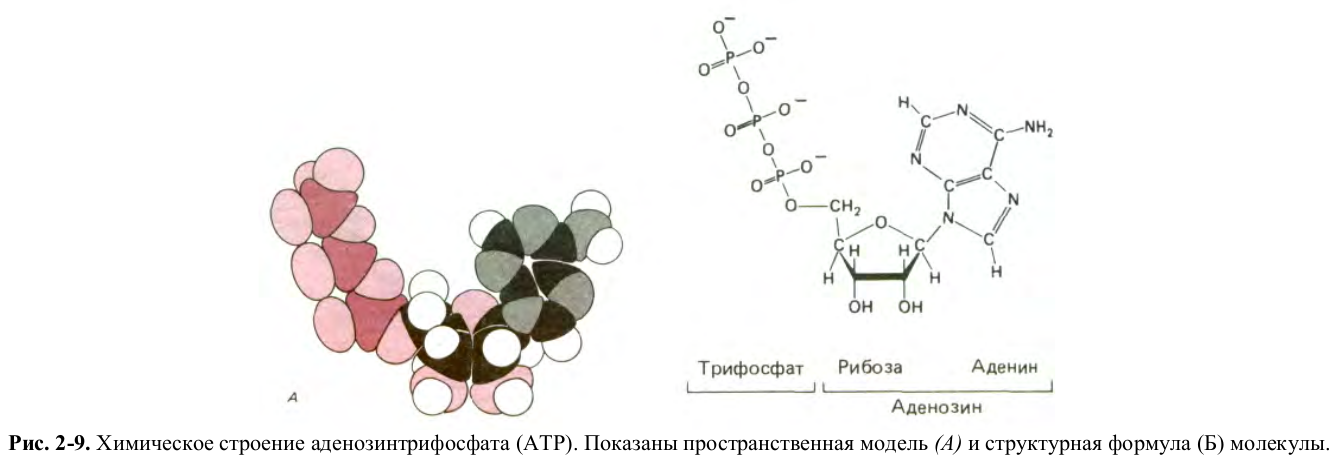
\includegraphics[scale=0.4]{2atf}
\end{figure}
Другие производные
нуклеотидов служат переносчиками отдельных химических групп, таких, как атомы водорода или остатки Сахаров, с одной молекулы на другую. Кроме того, циклическое фосфорилированное производное аденинациклический AMP (cAMP) -служит универсальным внутриклеточным сигналом и
регулирует скорость множества различных внутриклеточных реакций. \\

Нуклеотиды служат
строительными блоками для синтеза нуклеиновых кислот - длинных полимеров, в которых нуклеотидные субъединицы соединяются между собой
ковалентной связью, образуя фосфорный эфир между 3'-гидроксильной группой остатка сахара одного нуклеотида и 5'-фосфатной группой. Нуклеиновые кислоты, сахар которых представлен рибозой, называются рибонуклеиновыми кислотами или \textbf{РНК}; они
содержат основания A, U, G и С. Те нуклеиновые кислоты, в состав которых входит дезоксирибоза (в ней гидроксильная группа при С-2 рибозы
замещена на атом водорода), называются дезоксирибонуклеиновыми кислотами или \textbf{ДНК}; они содержат основания А, Т, G и С. Способность к спариванию G c C и A c T лежит в основе механизмов хранения и передачи наследственно информации.

\subsection{Формы ДНК}
Наиболее распространой является В-форма. В этой форме находится основная часть ДНК в клетках. При такой организации плоскости азотистых оснований практически перпендикулярны оси двойной спирали, и каждая пара повёрнута относительно предыдущих на $36^\circ$. На один виток спирали приходится примерно 10 нуклеотидных пар (9,7 и 10,6 в различных кристаллах)(2), а длина составляет 3,4 нм.
\begin{figure}[H]
	\centering
	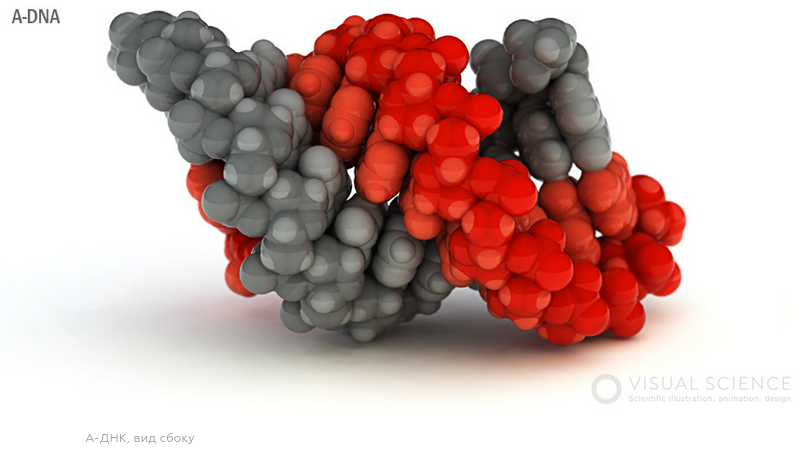
\includegraphics[scale = 0.5]{2adnk}
\end{figure}
Существенным отличием А-формы от В-формы является то, что в А-форме пары оснований сдвинуты к периферии спирали почти на половину её радиуса, в результате чего пространство вдоль оси оказывается пустым. Большая бороздка при этом становится глубже и уже, а малая бороздка оказывается шире и более плоской
\begin{figure}[H]
	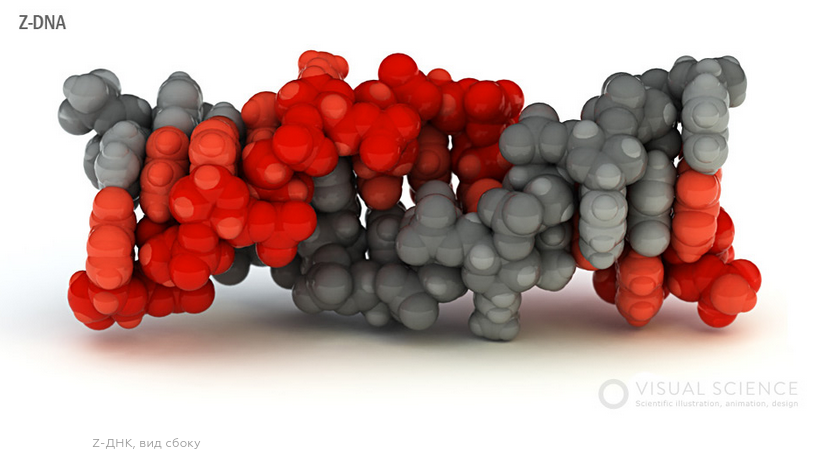
\includegraphics[scale=0.6]{2zdnk}
\end{figure} 
Z форма представляет собой левозакрученную спираль с длиной витка 4,4 нм, на который приходится 12 нуклеотидных пар.
\subsection{Отличие эукариот от прокариот}
Прокариоты не имеют оформленного ядра. Их хромосомы имеют кольцевую форму. А гены объеденены в опероны.
Эукариотические клетки по определению и в отличие от прокариотических имеют ядро (по гречески «карион»). Ядро, в котором
находится большая часть клеточной ДНК, ограничено двойной мембраной. 

\subsection{Генетический код}
\textbf{Генетичесий код - совокупность правил, согласно которым в живых клетках последовательность нуклеотидов (ген и мРНК) переводится в последовательность аминокислот (белок).}\\
Ген - участок днк определяющий определенную последовательность аминокислот.\\
Аллели - различные формы одного и того же гена, расположенные в одинаковых участках (локусах) гомологичных хромосом, определяют направление развития конкретного признака

\subsection{Митоз и мейоз}
Существует два типа деления клеток эукариот: митоз и мейоз. При митозе хромосомный набор (плоидность) клетки не меняется, обе дочерние клетки полностью генетически идентичны исходной. Это обычный способ деления клеток, например, при формировании тел многоклеточных животных и растений. В результате мейоза, который включает в себя 2 деления, из одной диплоидной клетки получается 4 гаплоидных, причем все они генетически отличаются друг от друга. Это может происходить при формировании гамет или спор.\\

\textbf{Мейоз} (редукционное деление клетки) — деление, в процессе которого из одной диплоидной клетки получаются 4 гаплоидные клетки.
\begin{figure}[H]
	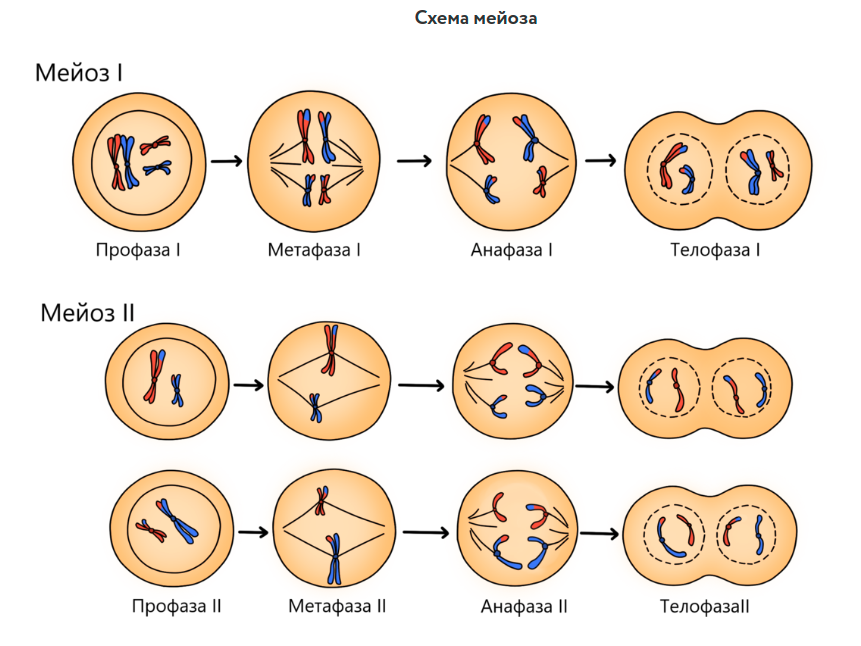
\includegraphics[scale=0.5]{2mi}
\end{figure}
Мейоз у животных наблюдается при формировании гамет (гаметогенезе). Мейоз у растений и грибов, как правило, происходит при образовании гаплоидных спор. У различных одноклеточных эукариот мейоз может наблюдаться на разных стадиях жизненного цикла. Для восстановления диплоидности в цикле всегда необходимо слияние гаплоидных клеток (оплодотворение).\\
Мейоз состоит из двух делений. Первое из них является собственно редукционным, то есть именно в ходе первого деления уменьшается плоидность клетки. Причиной этого служит расхождение гомологичных хромосом («материнской» и «отцовской») по двум разным дочерним клеткам. Второе деление аналогично митозу и называется эквационным (то есть «равным»). Плоидность в результате второго деления не меняется. В ходе этого деления, как и при митозе, расходятся сестринские хроматиды (копии ДНК). Между двумя делениями мейоза отсутствует репликация ДНК (так как «цель» мейоза — уменьшить плоидность клетки, увеличивать количество ДНК здесь незачем).\\
В профазе I деления мейоза происходит важнейший процесс, относящийся к генетической рекомбинации — кроссинговер, то есть обмен участками гомологичных хромосом.\\

\textbf{Митоз} - непрямое деление клетки, наиболее распространённый способ репродукции эукариотических клеток. Биологическое значение митоза состоит в строго одинаковом распределении хромосом между дочерними ядрами, что обеспечивает образование генетически идентичных дочерних клеток и сохраняет преемственность в ряду клеточных поколений. \textbf{Митоз лежит в основе бесполого размножения, от отличие от мейоза.}
\begin{figure}[H]
	\centering
	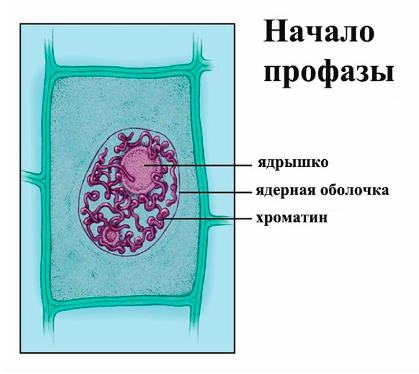
\includegraphics[scale = 0.5]{2m1}
	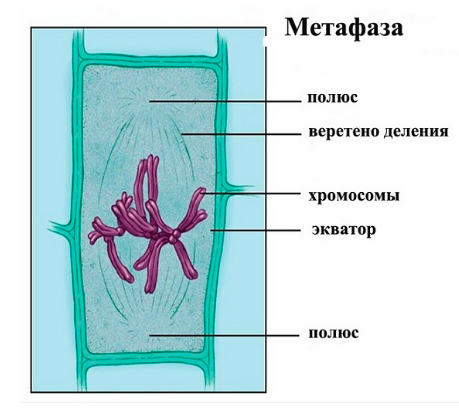
\includegraphics[scale = 0.5]{2m2}
	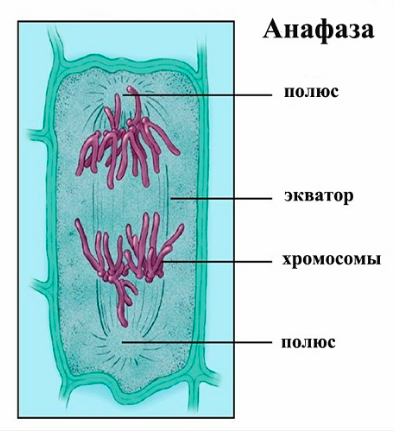
\includegraphics[scale = 0.5]{2m3}
	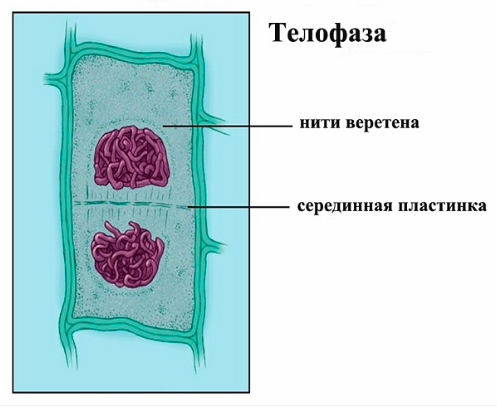
\includegraphics[scale = 0.5]{2m4}
\end{figure}
Профаза это подготовительный этап. ДНК удваивается и расходятся, они остаются соединены только в центромере. Образуется веретено деления. Микротрубочки веретена деления прикрепляются к хромосомам.\\
Затем наступает метафаза. За счет изменения длины нитей веретена хромосомы перемещаются в среднюю часть клетки, образуя экватор деления.\\
За метафазой наступает анафаза (см. рис. 6). Центромеры сестринских хроматид разделяются, нити веретена укорачиваются, в результате дочерние хроматиды расходятся к противоположным полюсам\\
Митоз завершается телофазой, в которой восстанавливается исходная структура ядер. Вокруг каждого набора хромосом у полюсов деления формируется новая ядерная оболочка
	
	\newpage
	
	\section{Репликация ДНК: репликация линейных и кольцевых молекул ДНК, 
Затравка для ДНК-полимеразы, праймирование, фрагменты Оказаки. 
Ферменты, необходимые для репликации ДНК (полимеразы I и III, топоизомеразы, хеликаза, лигаза, 
праймаза, ssb). 
Теломеры и центромеры эукариот. Ориджины репликации бактерий. Белки определяющие начало 
репликации бактерий (DnaABC, ssb, SeqA, dam) Репликация кольцевых молекул ДНК по Тета –типу и по типу катящегося колеса}


\textbf{Репликация ДНК} - процесс создания двух дочерних молекул ДНК на основе одной родительской молекулы ДНК. 

Двухцепочечная молекула ДНК может быть линейной (у эукариот, организмов, клетки которых имеют  клеточное ядро) или свернутой в кольцо (у прокариот, клетки которых не имеют ядра). 

Про особенности репликации двухцепочечных линейных и кольцевых молекул см. ниже.

\subsection{Общее описание механизма репликации}
Двухцепочечная молекула ДНК может быть линейной (у эукариот, организмов, клетки которых имеют  клеточное ядро) или свернутой в кольцо (у прокариот, клетки которых не имеют ядра). 

Про особенности репликации двухцепочечных линейных и кольцевых молекул см. ниже.

\subsection{Общее описание механизма репликации}
Что имеем в начале: клетка, у клетки есть ДНК. Клетка собирается делиться, ей надо \textbf{реплицировать} (скопировать) свою ДНК для двух дочерних клеток.

\begin{itemize}
    \item Репликация начинается в определенном месте материнской ДНК с расплетания топоизомеразой двойной спирали (см. рис. \ref{fig:3_replication_main}, \ref{fig:3_rep}).
    
    \item Хеликаза садится на выпрямленную двойную цепь ДНК и разделяет ее на две одиночные цепи ДНК. При этом формируется \textbf{репликационная вилка}. 
    
    \item SSB-белки (белки, связывающие одиночную цепь ДНК, англ. single-strand binding protein) удерживают две материнские цепи ДНК от связывания обратно. Получившаяся на этом этапе конструкция из ДНК и белков называется репликационной вилкой.
    
    \item К каждой из получившихся одиночных цепей ДНК теперь будет синтезироваться комплиментарная цепь из плавающих вокруг дезоксиробонуклеотидов.
    
    \item \textbf{Процесс на лидирующей цепи  3'-5'}. Праймаза ставит на цепь 3'-5' (относительно направления расплетания двойной цепи) праймер - РНК-затравку для посадки ДНК-полимеразы. Садится ДНК-полимераза и едет по материнской цепи ДНК, синтезируя комплементарную ей цепь из свободно плавающих нуклеотидов. ДНК-полимераза умеет присоединять только 5' конец предыдущего дезоксирибонуклеотида к 3' концу следующего дезоксирибонуклеотида. 
    
    \item \textbf{Процесс на отстающей цепи 5'-3'}. Праймаза ставит праймер для полимеразы. ДНК-полимераза садится на него и синтезирует небольшой фрагмент ДНК (\textbf{фрагмент Оказаки}) в обратном направлении относительно расплетания материнской ДНК. Фрагменты Оказаки сшиваются лигазой.
    
    \item В итоге имеем две дочерние двунитевые молекулы ДНК вместо одной материнской.
    
\end{itemize}

Репликационная вилка движется со скоростью порядка 100 000 пар нуклеотидов в минуту у прокариот и 500—5000 — у эукариот.

\begin{figure}[H]
    \centering
    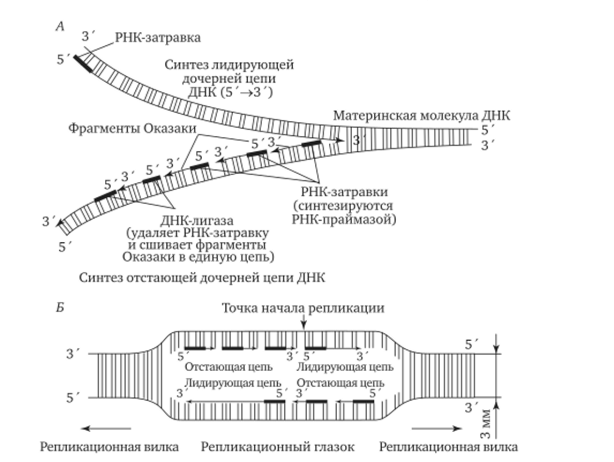
\includegraphics[width = 0.8 \linewidth]{3_replication_main.png}
    \caption{Схема репликационной вилки (выше) и репликационного глазка (ниже). Репликационная вилка на втором рисунке - область, где материнская двухцепочечная молекула расходится на две. Стрелочками обозначено то, что вилки удаляются друг от друга, двигаясь по материнской (шаблонной) ДНК в направлении от 3' к 5' концам.}
    \label{fig:3_replication_main}
\end{figure}

\subsection{Ферменты, необходимые для репликации ДНК}

\begin{itemize}

    \item \textbf{Топоизомераза} - фермент, раскручивающий спираль ДНК. Едет вдоль закрученной двойной спирали ДНК и ставляет за собой две водородно связанные цепочки ДНК, лежащие в одной плоскости. (здесь и далее смотреть на картинку \ref{fig:3_rep}).
    
    \item \textbf{Хеликаза} - фермент, рвущий водородные связи между двумя цепочками ДНК. Едет за топоизомеразой по двум связанным цепям ДНК и оставляет за собой две несвязанные цепи ДНК.
    
    \item \textbf{Полимераза} (ДНК полимераза) - фермент, полимеризующий молекулу ДНК. Всегда едет по цепи ДНК в направлении 3'-5', смотрит на нее как на шаблон и достраивает комплиментарную ей цепь из свободно плавающих дезоксирибонулеотидов. 
    
    ДНК-полимераз существует несколько типов. У бактерий \textbf{ДНК-полимераза I} удаляет РНК-фрагменты на отстающей цепи и ставит на их место ДНК, \textbf{ДНК-полимераза II} участвует в репарации (восстановлении сломанных кусочков) ДНК, \textbf{ДНК-полимераза III} просто основной фермент (именно она делает почти всю работу в синтезировании ДНК с лидирующей и отстающей цепей).
    
    \item \textbf{Лигаза} (ДНК-лигаза) - фермент, ковалентно сшивающий цепи ДНК в местах разрыва. Едет по отстающей цепи ДНК и сшивает фрагменты ОКазаки. 
    
    \item \textbf{Праймаза} - фермент, синтезирующий РНК-затравку (праймер) — короткий фрагмент РНК, которая является инициатором в работе ДНК-полимеразы (полимераза не способна синтезировать ДНК с нуля, но может добавлять нуклеотиды к уже имеющимся). 
    
    \item \textbf{SSB-белки} - ферменты, предотвращающие диссоциацию полимеразы от матрицы ДНК и повышающие эффективность ее работы. Окружают кольцом ДНК и «скользят» по ней вместе с продвигающимся вперед ферментом ДНК-полимеразы. 
    
    \begin{figure}[H]
        \centering
        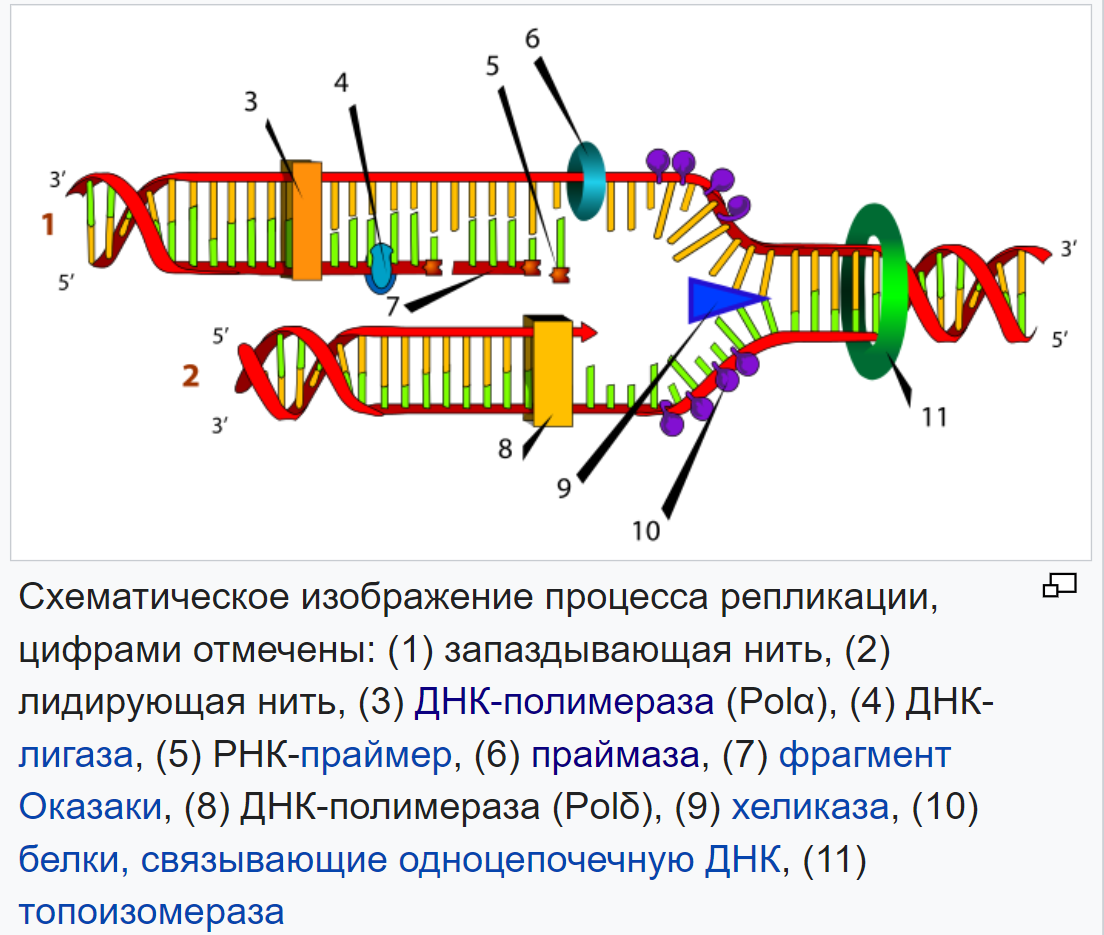
\includegraphics[width=0.7\linewidth]{3_replication.png}
        \caption{Белки, участвующие в процессе репликации}
        \label{fig:3_rep}
    \end{figure}
    
\end{itemize}

\subsection{Теломеры и центромеры эукариот}
\textbf{Теломеры} - концевые участки хромосом. Теломерные участки хромосом характеризуются отсутствием способности к соединению с другими хромосомами или их фрагментами и выполняют защитную функцию. 

В каждом цикле деления теломеры клетки укорачиваются из-за неспособности ДНК-полимеразы синтезировать копию ДНК с самого конца. Она в состоянии лишь добавлять нуклеотиды к уже существующей 3’-гидроксильной группе. Данный феномен носит название концевой недорепликации и является одной из важнейших причин биологического старения.

Тем не менее, вследствие этого явления теломеры должны укорачиваться весьма медленно — по несколько (3-6) нуклеотидов за клеточный цикл.

\begin{figure}[H]
    \centering
    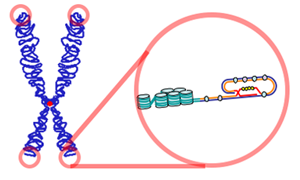
\includegraphics[]{3_telomere.png}
    \caption{Концевые участки хромосом, теломеры}
    \label{fig:3_telomere}
\end{figure}

\textbf{Центромеры} - участок хромосомы, который связывает сестринские хроматиды, играет важную роль в процессе деления клеточного ядра и участвует в контроле экспрессии генов. Характеризуется специфическими последовательностью нуклеотидов и структурой.

\begin{figure}[H]
    \centering
    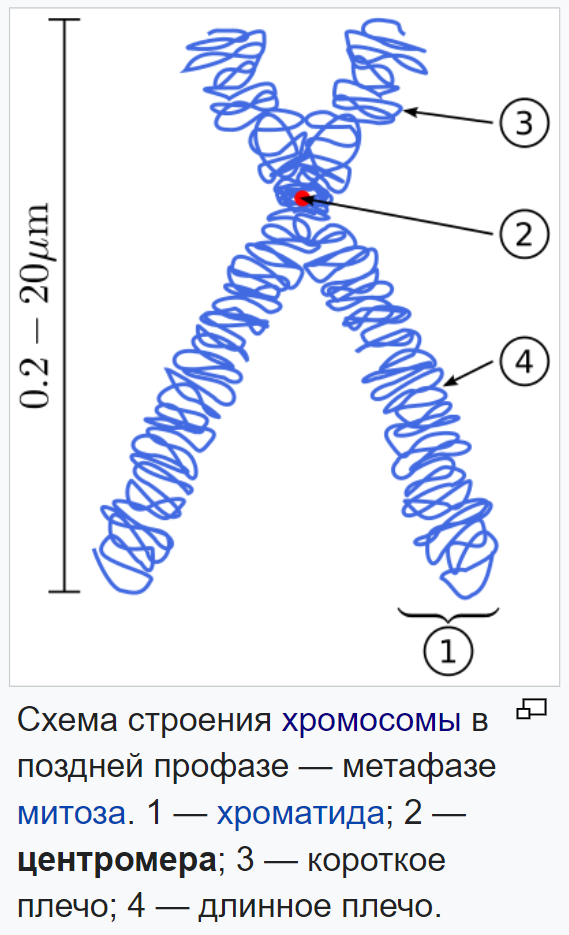
\includegraphics[width = 0.3 \linewidth]{3_centromere.png}
    \caption{Центральные участки хромосом, центромеры}
    \label{fig:3_centromere}
\end{figure}

\subsection{Ориджины репликации у бактерий}
\textbf{Точка начала репликации} (англ. origin of replication) — это фрагмент молекулы нуклеиновой кислоты, с которого начинается её репликация. Точка начала репликации и прилегающие к ней фрагменты нуклеиновой кислоты, не отделённые сайтами терминации, составляют единицу репликации — репликон. Репликация ДНК может начинаться от точки начала репликации в одном или двух направлениях.

Хромосомы и плазмиды (внехромосомный самовоспроизводящийся генетический элемент, специфичен для прокариот) прокариот (в частности, бактерий) содержат одну, реже несколько точек начала репликации ДНК (хромосомы эукариот имеют множество таких точек).

\subsection{Белки, определяющие начало репликации у бактерий}

Проиллюстрируем на примере Escherichia coli.

Генетический локус, содержащий единственную точку начала репликации хромосомы Escherichia coli (кишечной палочки), получил название oriC. OriC состоит из 245 пар оснований и включает две функциональных области: область специфичного связывания фактора инициации репликации DnaA (англ.) и область первичного раскручивания спирали ДНК — DUE (англ. DNA unwinding element). 

\subsection{Репликация кольцевых молекул ДНК по тета-типу}
Репликация по тета-механизму включает в себя следующие этапы:
\begin{itemize}
    \item 
    расплетание двух родительских цепей;
    \item
    синтез праймерной РНК (пРНК) на каждой из них;
    \item
    инициация репликации при помощи ковалентного нарастания пРНК на каждой из них;
    \item
    синтез комплементарной цепи ДНК на каждой из родительских цепей. Одна из цепей при этом выступает лидирующей, другая — отстающей, хотя синтез цепей происходит одновременно.
\end{itemize}

Тета-репликация может начинаться одновременно с одной или нескольких точек и быть при этом одно- или двунаправленной. В электронный микроскоп репликационная структура выглядит как греческая буква \(\theta\), отчего и называется тета-структурой (см. рис. \ref{fig:3_theta}).

\begin{figure}[H]
    \centering
    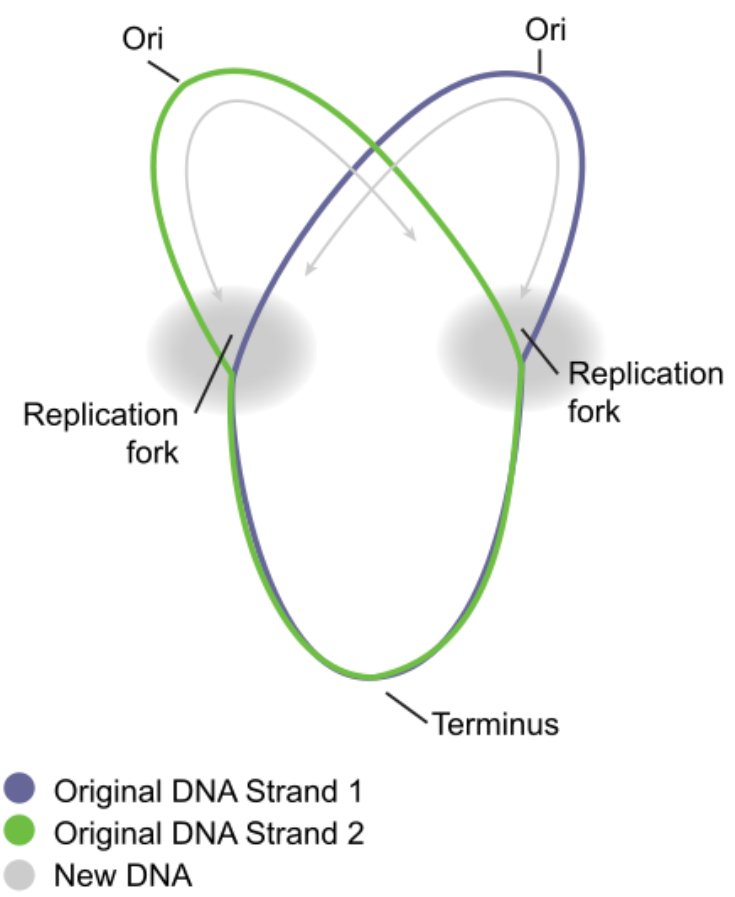
\includegraphics[width = 0.4 \linewidth]{3_theta.png}
    \caption{Этап репликации по тета-типу. Видно две репликационные вилки, разъезжающиеся друг от друга (показано стрелочками). Ori - место начала репликации (ориджин).}
    \label{fig:3_theta}
\end{figure}

\subsection{Репликация кольцевых молекул ДНК по типу катящегося колеса}
Сущность этого механизма заключается в следующем. Вначале инициаторный белок Rep совершает одноцепочечный разрыв в цепи ДНК. Появившаяся при этом свободная 3'-OH-группа служит праймером для синтеза ДНК ДНК-полимеразой III клетки-хозяина. Cинтезируется лидирующая цепь и восстанавливается двухцепочечная структура исходной ДНК. Содержащая разрыв цепь ДНК при этом удаляется, и происходит её репликация ДНК-полимеразой III, сопровождающаяся созданием праймера РНК-полимеразой. После полной репликации ДНК-полимераза I заменяет праймер на ДНК, а ДНК-лигаза сшивает концы, образуя тем самым окончательную двухцепочечную ДНК (см. \ref{fig:3_wheel}).

\begin{figure}[H]
    \centering
    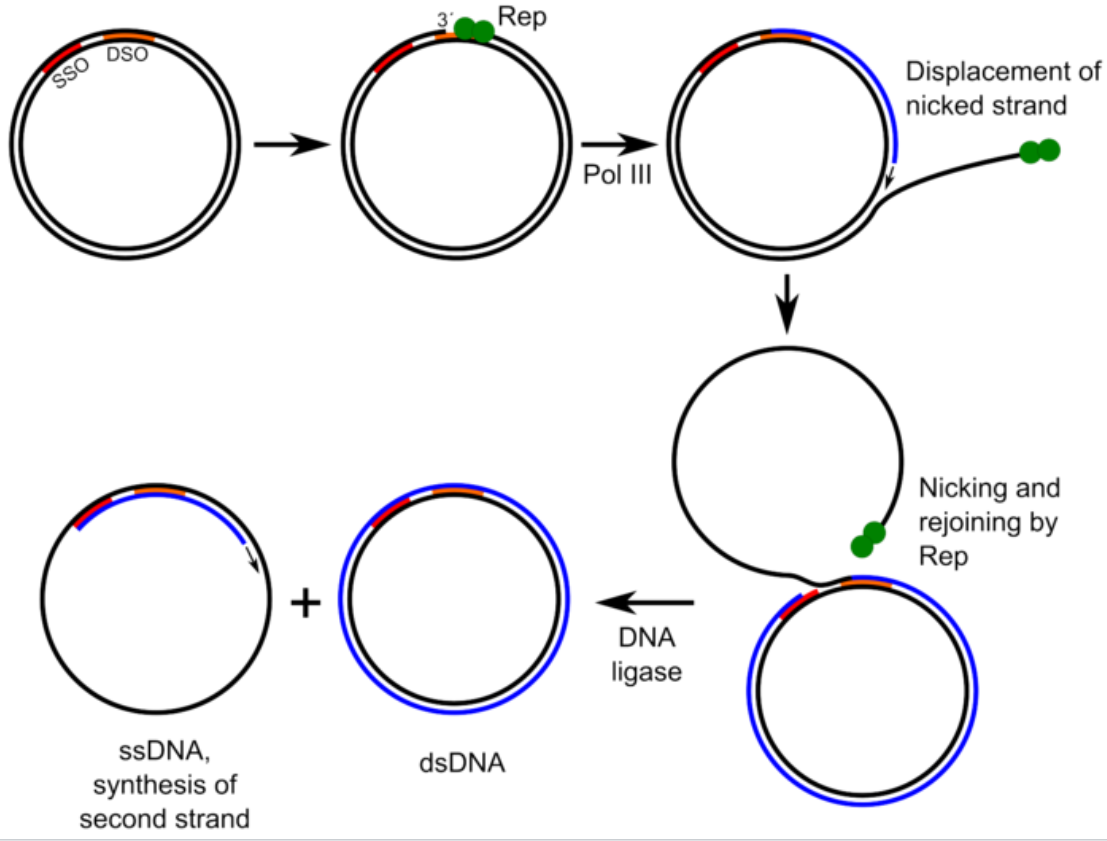
\includegraphics[width = 0.6 \linewidth]{3_wheel.png}
    \caption{Этапы репликации по типу катящегося колеса}
    \label{fig:3_wheel}
\end{figure}

	
	\newpage
	
	\input{TeX_files/4.tex}
	
	\newpage
	
	\section{Трансляция}

Простыми словами: процесс, при котором рибосома синтезирует белок\footnote{Цепочка аминокислот} на основе кодонов\footnote{Триплет нуклеотидов, например, GUC} матричной РНК(мРНК). 

Сложными словами: процесс считывания информации с мРНК при помощи адапторных молекул тРНК и катализ образования пептидных связей между присоединёнными к тРНК аминокислотами.

 


Трансляция состоит из 3 этапов: 

\begin{itemize}
    \item Инициация -- Узнавание стартового кодона (AUG), присоединение тРНК и объединение большой и малой субъединиц рибосомы.
    \item Элонгация -- Узнавание текущего кодона соответствующей ему аминоацил-тРНК; присоединение аминокислоты, принесённой тРНК, к концу растущей полипептидной цепи; продвижение рибосомы вдоль матрицы, сопровождающееся высвобождением молекулы тРНК; 
    аминоацилирование высвободившейся молекулы тРНК соответствующей ей аминоацил-тРНК-синтетазой;  присоединение следующей молекулы аминоацил-тРНК; движение рибосомы по молекуле мРНК до стоп-кодона.
    \item Терминация: Синтез белка продолжается до тех пор, пока на рибосоме не окажется один из трёх стоп-кодонов (УАА, УАГ или УГА). После этого белковая цепочка отсоединяется от рибосомы, выходит в цитоплазму и формирует присущую этому белку вторичную, третичную и четвертичную структуры.
\end{itemize}

\begin{figure}[h]
    \centering
    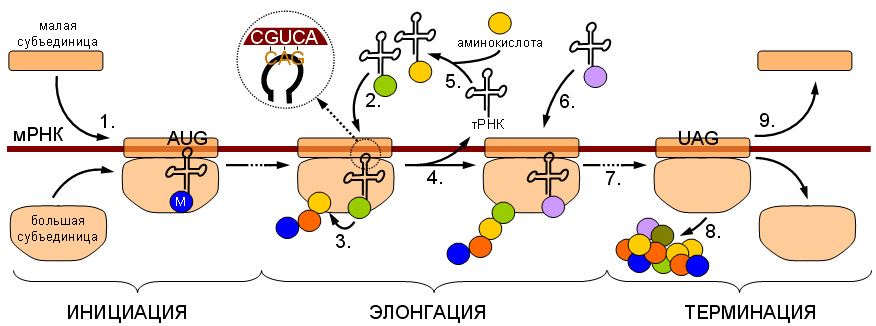
\includegraphics[width=0.8\textwidth]{Pictures/5_3(translation_e).jpg}
    \caption{Схема трансляции}
    \label{fig:5_3(translation_e)}
\end{figure}


\subsection{Структура рибосомы. Рибосомная РНК и белки}

\Def{Рибосома}(от «РНК» и soma – тело) -- клеточный немембранный\footnote{Немембранные органеллы лишены собственной замкнутой мембраны и не имеют четкой границы с цитоплазмой.} органоид, осуществляющий трансляцию (считывание кода мРНК и синтез полипептидов).  Присутствует у всех живых организмов, находится в жидкой внутренней среде клетки -- цитоплазме(рис. \ref{fig:5_1(cells)}). Состоит из рРНК(рибосомных РНК) и р-белков. 

По строению рибосома состоит из двух субъединиц: малой (1 молекула рРНК и 33 белка) и большой (3 молекулы рРНК и 40 белков), которые  соединяются вместе только на молекуле мРНК для синтеза белка. Малая субъединица считывает информацию с матричной РНК, а большая — присоединяет соответствующую аминокислоту к синтезируемой цепочке белка (рис. \ref{fig:5_24}). Массы субъединиц выражаются в измеряемых напрямую константах седиментации (скорость осаждения в единицах Сведберга, S)

\begin{figure}[h]
    \centering
    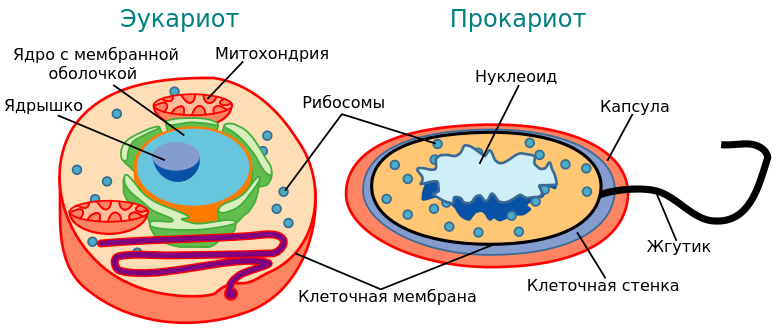
\includegraphics[width=0.7\textwidth]{Pictures/5_1(cell)}
    \caption{Строение клетки}
    \label{fig:5_1(cells)}
\end{figure}

Рибосомы в клетках эукариот состоят из четырех нитей РНК (три молекулы рРНК в большой субъединице и одна молекула рРНК – в малой) и примерно 80 разных белков, т.е представляют собой сложнейший комплекс из молекул, скрепленных слабыми, нековалентными связями. Рибосомы в клетках прокариот состоят из трех нитей РНК; две нити рРНК находятся в большой субъединице и одна рРНК – в малой. 

рРНК синтезируются РНК-полимеразой I в виде длинной молекулы пред-рибосомальной РНК, которая разрезается на отдельные РНК, составляющие основу рибосом.

\subsection{Функциональные активности и функциональные участки рибосомы}

Рибосома в процессе трансляции выполняет следующие функции:  

\begin{itemize}
    \item Связывание  и удержание  матричного полинуклеотида  (мРНК-связывающий участок)
    
    \item Удержание  пептидил-тРНК    или   деацилированной тРНК  (тРНК-связывающий  Р-участок);
    
    \item Связывание  аминоацил-тРНК  (тРНК-связывающий А-участок);
    
    \item Связывание  белковых  факторов  трансляции  и  ГТФ (факторсвязывающий  участок);
    
    \item Участие в катализе гидролиза ГТФ;
    
    \item Катализ транспептидации -- процесса, при котором аминокислота прикрепляется к хвосту уже собранного белка.
    
    \item Транслокация -- перемещение рибосомы по мРНК на один триплет.
\end{itemize}



\begin{figure}[h]
\begin{minipage}[h]{0.5\linewidth}
\center{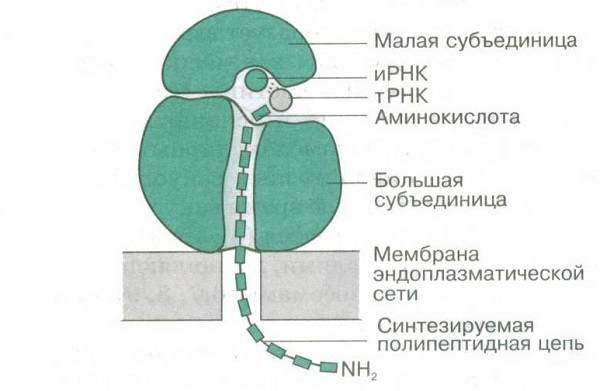
\includegraphics[width=0.7\linewidth]{Pictures/5_2(rybosome).jpg} \\ а)}
\end{minipage}
\hfill
\begin{minipage}[h]{0.5\linewidth}
\center{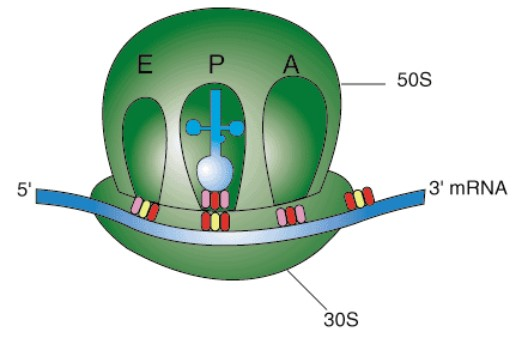
\includegraphics[width=0.6\linewidth]{Pictures/5_4(sites).jpg} \\ б)}
\end{minipage}
\caption{Строение рибосомы: а) расположение субъединиц б) расположение функциональных участков}
\label{fig:5_24}
\end{figure}


В процессе элонгации участие два белковых фактора. Первый переносит аминоацилированную («заряженную» аминокислотой) тРНК в А (аминоацил)-сайт рибосомы(рис. \ref{fig:5_24}б). Рибосома катализирует перенос пептида, связанного с тРНК в Р-сайте, в А-сайт и образование пептидной связи с находящимся там аминокислотным остатком(то есть тРНК "приносит" часть белка, а рибосома присоединяет его к строящейся цепочке). Таким образом растущий пептид удлиняется на один аминокислотный остаток. 

Затем второй белок катализирует транслокацию — перемещение рибосомы по мРНК на один триплет, в результате которого пептидил-тРНК оказывается вновь в Р-сайте, а «пустая» тРНК из P-сайта переходит в Е-сайт (от слова exit). тРНК из E-сайта диссоциирует спонтанно, после чего рибосома готова к новому циклу элонгации.

\subsection{Информационные и транспортные РНК. Аминоацил-тРНК-синетазы}

\Def{Информационная(=матричная) РНК}
Поскольку прокариотическая мРНК не нуждается в обработке и транспортировке, трансляция рибосомой может начаться немедленно после транскрипции. Следовательно, можно сказать, что трансляция у прокариот совмещена с транскрипцией и происходит ко-транскрипционно.

Эукариотическая мРНК должна быть обработана и доставлена из ядра в цитоплазму, и только тогда может быть транслирована рибосомой. Трансляция может происходить как на рибосомах, находящихся в цитоплазме в свободном виде, так и на рибосомах, ассоциированных со стенками эндоплазматического ретикулума. Таким образом, у эукариот трансляция не совмещена напрямую с транскрипцией. 

\Def{Транспортные РНК}
Одноцепочечная последовательность в форме листа клевера. Она формирует одноцепочечный участок, который заканчивается последовательностью ЦЦА со свободной ОН-группой. К этому концу присоединяется транспортируемая аминокислота. 3 остальные части представляют собой комплементарно спаренные последовательности нуклеотидов, которые заканчиваются неспаренными участками, образующими петли.

\Def{Аминоацил-тРНК-синетаза}
Транспортная тРНК(61 вид) и соответствующая ец аминокислотаа(20 видов) соединяются с помощью специального белка -- Аминоацил-тРНК-синетазы. Аминоацил = кислотный остаток, синтетаза = белок, синтезирующий что-то. К 3' концу тРНК прицепляется аминокислота и белок отделяется.

\subsection{Энергетика биосинтеза белка, использование АТФ и ГТФ}

Синтез белка -- энергозатратный процесс. Энергия на создание связи между тРНК и аминокислотой берется из гидролиза нуклеозидтрифосфатов АТФ и ГТФ.

Аминокислота активируется с использованием АТФ и присоединяется к тРНК с помощью фермента аминоацил-тРНК-синтетазы.

\Def{АТФ}
(Аденозинтрифосфат) -— нуклеозидтрифосфат.  

АТФ относится к так называемым макроэргическим соединениям, то есть к химическим соединениям, содержащим связи, при гидролизе которых происходит освобождение значительного количества энергии. Гидролиз макроэргических связей молекулы АТФ, сопровождаемый отщеплением 1 или 2 остатков фосфорной кислоты, приводит к выделению, по различным данным, от 40 до 60 кДж/моль. 

Подробнее в следующем разделе и на рис. \ref{fig:5_6(init_pro)}

\subsection{Инициация трансляции у прокариот, последовательность Шайна-Далгарно}


Первую фазу трансляции — инициацию — можно разделить на несколько стадий. На первой стадии два белковых фактора инициации IF-1 и IF-3 связываются с 30S-субчастицей (рис. \ref{fig:5_6(init_pro)}(1)). Затем еще один белковый фактор, IF-2, образует комплекс с ГТФ (GTP) (рис. \ref{fig:5_6(init_pro)}(2)), что облегчает ассоциацию 30S-субчастицы с мРНК (mRNA) и связывание тРНК (tRNA), соответствующей инициирующему кодону (рис. \ref{fig:5_6(init_pro)}(3)). У прокариот стартовая тРНК несет N-формилметионин (f-Met), у эукариот — метионин. В завершение 50S-субчастица связывается с вышеупомянутым комплексом (рис. \ref{fig:5_6(init_pro)}(4)). На третьей и четвертой стадиях идет освобождение факторов инициации и гидролиз связанного с IF-2 ГТФ до ГДФ (GDP) и неорганического фосфата Р. Таким образом, связанный с 70S-рибосомой инициирующий комплекс содержит формилметионин-тРНК в тРНК-связывающем участке, называемом пептидильным участком (Р). Второе место связывания, акцепторный участок (А), во время этой фазы трансляции остается свободным.

\begin{figure}[h]
    \centering
    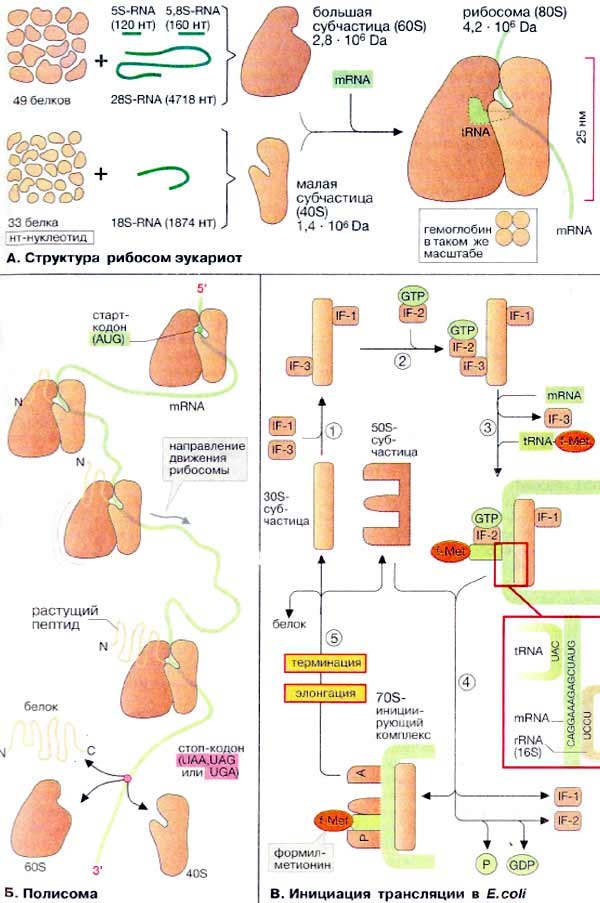
\includegraphics[width=0.5\textwidth]{Pictures/5_6(init_pro).jpg}
    \caption{Трансляция у прокариот на примере E.coli}
    \label{fig:5_6(init_pro)}
\end{figure}

\Def{Последовательность Шайна — Дальгарно} 
-- сайт связывания рибосом AGGAGG на молекуле мРНК прокариот, обычно на расстоянии около 10 нуклеотидов до стартового кодона AUG; в случае E. coli последовательность Шайна — Дальгарно — AGGAGGU. Комплементарная последовательность CCUCCU, называемая последовательностью анти-Шайна — Дальгарно, располагается на 3'-конце молекулы 16S рибосомной РНК. Комплементарное взаимодействие между последовательностями Шайна — Дальгарно и анти-Шайна — Дальгарно служит для помещения старт-кодона мРНК в P-сайт рибосомы для начала биосинтеза белка.

\subsubsection{Терминация трансляции прокариот}

Факторы терминации:

\begin{itemize}
    \item RF-1 вызывает отделение полипептидной цепи при считывании кодонов UAA и UAG;
    \item RF-2 действует аналогичным образом при считывании UAA и UGA;
    \item EF-3 может облегчить работу двух других факторов.
\end{itemize}

Этапы терминации трансляции прокариот:

\begin{itemize}
    \item В А-участке оказывается один из трех терминирующих кодонов –UAG, UAA или UGA;
    \item Из-за отсутствия тРНК, отвечающих этим кодонам,полипептидил-тРНКостается связанной с Р-участком RF-1 и RF-2 катализируют отсоединение полипептидной цепи от тРНК, отделение их обоих от рибосомы, а 70S-рибосомы –от мРНК;
    \item RF-1 узнает в А-участке кодон UAA или UAG•RF-2 включается в том случае, когда в А-участке оказывается UAA или UGA;
    \item RF-3 облегчает работу двух других факторов;
    \item Если терминирующим кодоном является UAA, то эффективность процесса терминацииоказывается наибольшей, поскольку этот кодон узнают оба фактора –RF-1 и RF-2.
\end{itemize}

\subsection{Инициация трансляции у эукариот, кэп-сайт.Терминация трансляции.}

Кэп представляет собой модифицированный рибонуклеотид — 7-метилгуанозин, соединённый 5'-трифосфатным мостиком с первым нуклеотидным остатком транскрипта. Кэп способствует эффективному процессингу пре-мРНК, экспорту мРНК из ядра, её трансляции и защите от быстрой деградации.

У эукариот старт-сайтом трансляции обычно (но не всегда) является AUG кодон.
Консенсусная последовательность Козак, играющая важную роль в инициации трансляции у эукариот, включает 4-6 нуклеотидов, предшествующих старт-кодону, и 1-2 нуклеотида непосредственно после старт-кодона. 

Оптимальный нуклеотидный контекст AUG кодона, коррелирует с высоким уровнем синтеза белка ссоответствующей мРНК in vivo и является характеристикой так называемой "сильной" (эффективно инициирующей трансляцию) последовательности Козак.

Последовательность Козак не является сайтом связывания рибосомы, в отличие от прокариотической последовательности Шайна-Дальгарно.

\begin{figure}[h]
    \centering
    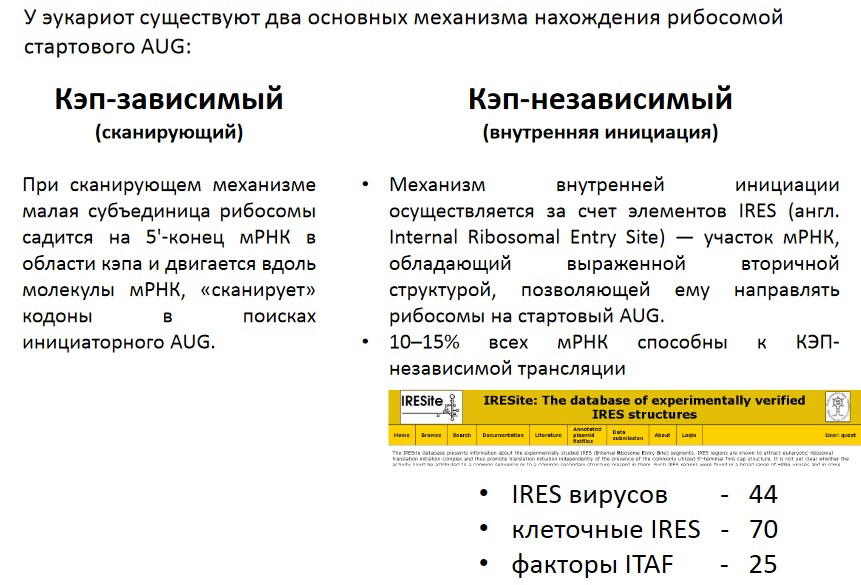
\includegraphics[width=0.7\textwidth]{Pictures/5_5(init_eu).jpg}
    \caption{Типы инициации трансляции эукариот}
    \label{fig:5_5(init_eu)}
\end{figure}

\subsubsection{Терминация трансляции эукариот}

Терминация происходит аналогично прокариотам. Терминация белкового синтеза у эукариот требует по крайней мере двух белков (eRF's от eukaryotic release factors), eRF1 и eRF3.
	
	\newpage
	
	\section{Репликоны.
Инициация раунда репликации ДНК Escherichia coli. Белки участвующие в регуляции инициации 
репликации (DnaABC, ssb, SeqA, dam).
Топологические проблемы репликации. Сегрегация репликонов по бактериальным клеткам.
Репликация плазмид, мобильных элементов, фагов и вирусов.
Особенности репликации в эукариотах. Теломеры и центромеры. Сегрегация хромосом.}

\subsection{Репликоны}

\textbf{Репликон} — молекула или участок ДНК или РНК, реплицирующийся из одного места начала репликации.

Задача: реплицировать ДНК. 

Как ее можно решать: посадить белки в одном месте и проехаться ими по всей ДНК (бактерии) или распараллелить процесс, посадив много белков в разных местах (эукариоты).

Например, у прокариот кольцевая ДНК имеет одну точку начала репликации, таким образом, она вся - репликон (см. рис. \ref{fig:6_replicon2}). У эукариот длинная линейная ДНК имеет множество точек начала репликации, то есть у нее много репликонов (см. рис. \ref{fig:6_replicon2}, \ref{6_replicon1}).

\begin{figure}[h!]
    \centering
    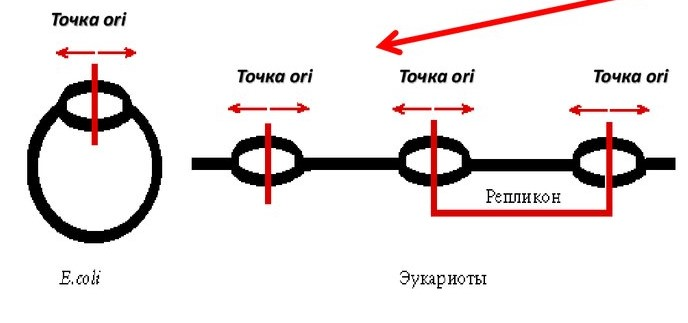
\includegraphics{6_replicon2.jpg}
    \caption{Иллюстрация репликонов бактерий и эукариотов. Слева - кольцевая ДНК кишечной палочки, у нее одно место начала (ori) репликации и она сама один репликон. Саправа - линейная ДНК эукариот со множеством репликонов. Стрелочками обозначены движения репликационных вилок.}
    \label{fig:6_replicon2}
\end{figure}

\begin{figure}
    \centering
    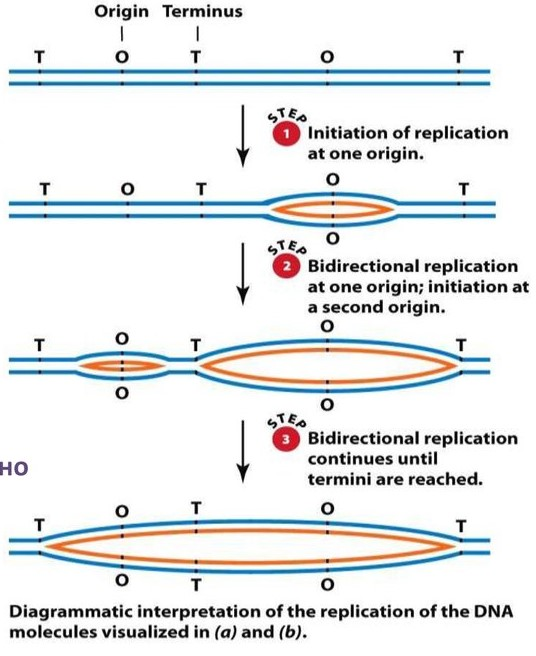
\includegraphics[width = 0.5 \linewidth]{6_replicon1.jpg}
    \caption{Репликоны эукариот - участки от O (origin) до T (termini).}
    \label{fig:6_replicon1}
\end{figure}

\subsection{Инициация раунда репликации ДНК Escherichia coli. Белки участвующие в регуляции инициации 
репликации (DnaABC, ssb, SeqA, dam).}

Здесь мы рассмотрим подробно процесс запуска репликации ДНК кишечной палочки с перечислением некоторых конкретных белков. (Подробнее о репликации см. билет 3.)

Имеется кольцевая двухцепочечная молекула ДНК со специальной точкой (читай, местом) начала репликации OriC. Клетка набрала достаточную массу для начала деления. 

\begin{itemize}
    \item Белки dnaA узнают OriC, садятся на ДНК и начинают раскручивать его. То есть, если смотреть на принципиальную схему репликации (билет 3, рис. \ref{fig3:rep}), dnaA является топоизомеразой кишечной палочки.
    
    \item Белок dnaC помогает белку dnaB сесть на ДНК и начать его разделять на две несвязанные цепи в том месте, где его расплела dnaA. Таким образом, dnaB - хеликаза кишечной палочки.
    
    \item SSB-белки удерживают две цепи ДНК, разделенные dnaB, от обратного связывания друг с другом.
    
    \item SeqA - белок, который садится на ДНК в области oriC после инициации репликации и не подпускает остальные белки для повторной инициации (потому что задача синтезировать две двухцепочечные молекулы ДНК из одной и распределить их по дочерним клеткам, а не размножать ДНК в геометрической прогрессии, пока у клетки не кончатся ресурсы).
    
    \item Dam - приходит на место посадки SeqA и <<обрабатывает>> (метилирует аденин) новые дочерние цепи ДНК так, чтобы на них dnaA не садилась уже по умолчанию (до тех пор, пока дочерняя клетка не вырастет), а не только пока их область OriC закрыт белками SeqA.
\end{itemize}

\subsection{Топологические проблемы репликации.}

При удвоении кольцевой ДНК бактерий могут получиться два кольца, сцепленных друг с другом (см. рис. \ref{fig:6_topology}). Их разделение производит топоизомераза II, или гираза. Она делает разрыв, через который проводит двухцепочечную нить ДНК, и снова сшивает.

\begin{figure}[h!]
    \centering
    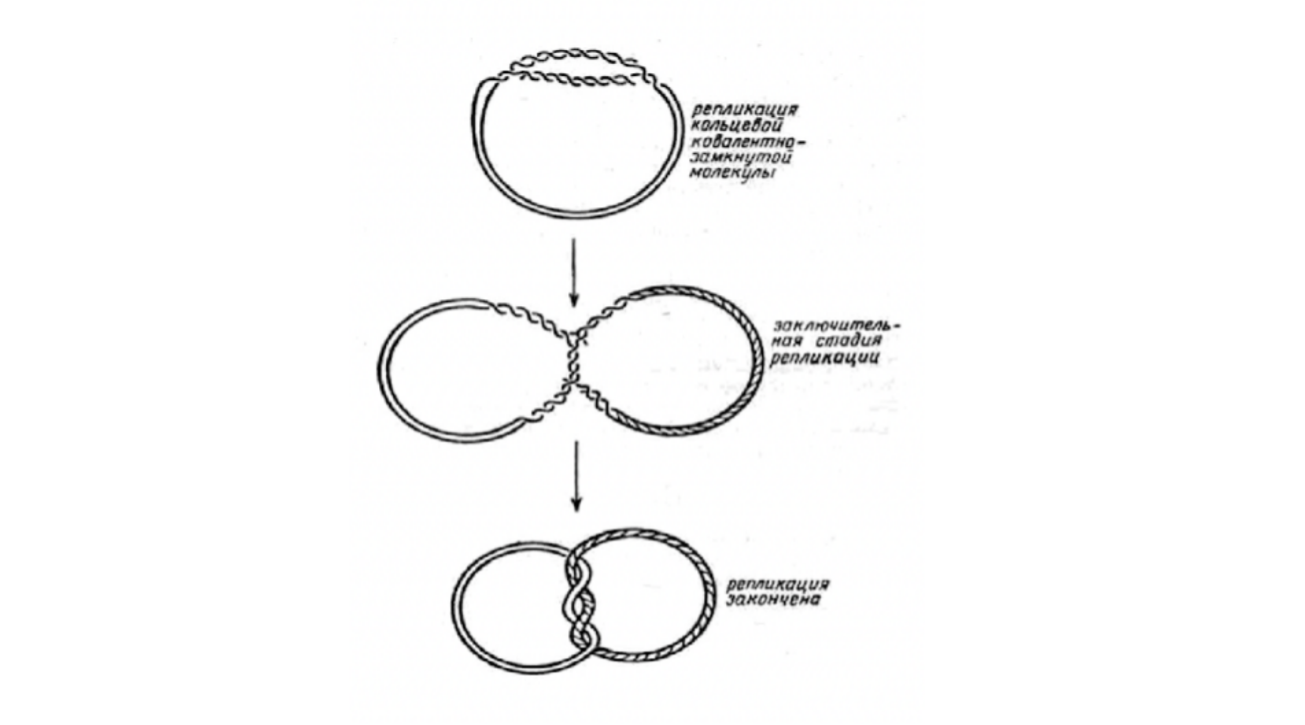
\includegraphics[width = 0.8 \linewidth]{6_topology.png}
    \caption{Топологические проблемы репликации кольцевых молекул ДНК (на две материнских цепи ДНК в кольце тоже переплетены ирл, просто для упрощения восприятия их так нарисовали).}
    \label{fig:6_topology}
\end{figure}

\subsection{Сегрегация репликонов по бактериальным клеткам.}

Прокариоты, в отличие от эукариот, не имеют такого сложного механизма деления клетки (см. билет про метоз и мейоз и сравнить с картинкой \ref{fig:6_deleniye}). Например, у них не образуется стадии <<веретена>>. Конкретный механизм сегрегации хромосом (одна хромосома у прокариот является также репликоном, см. параграф выше) не описан. 

\begin{figure}[h!]
    \centering
    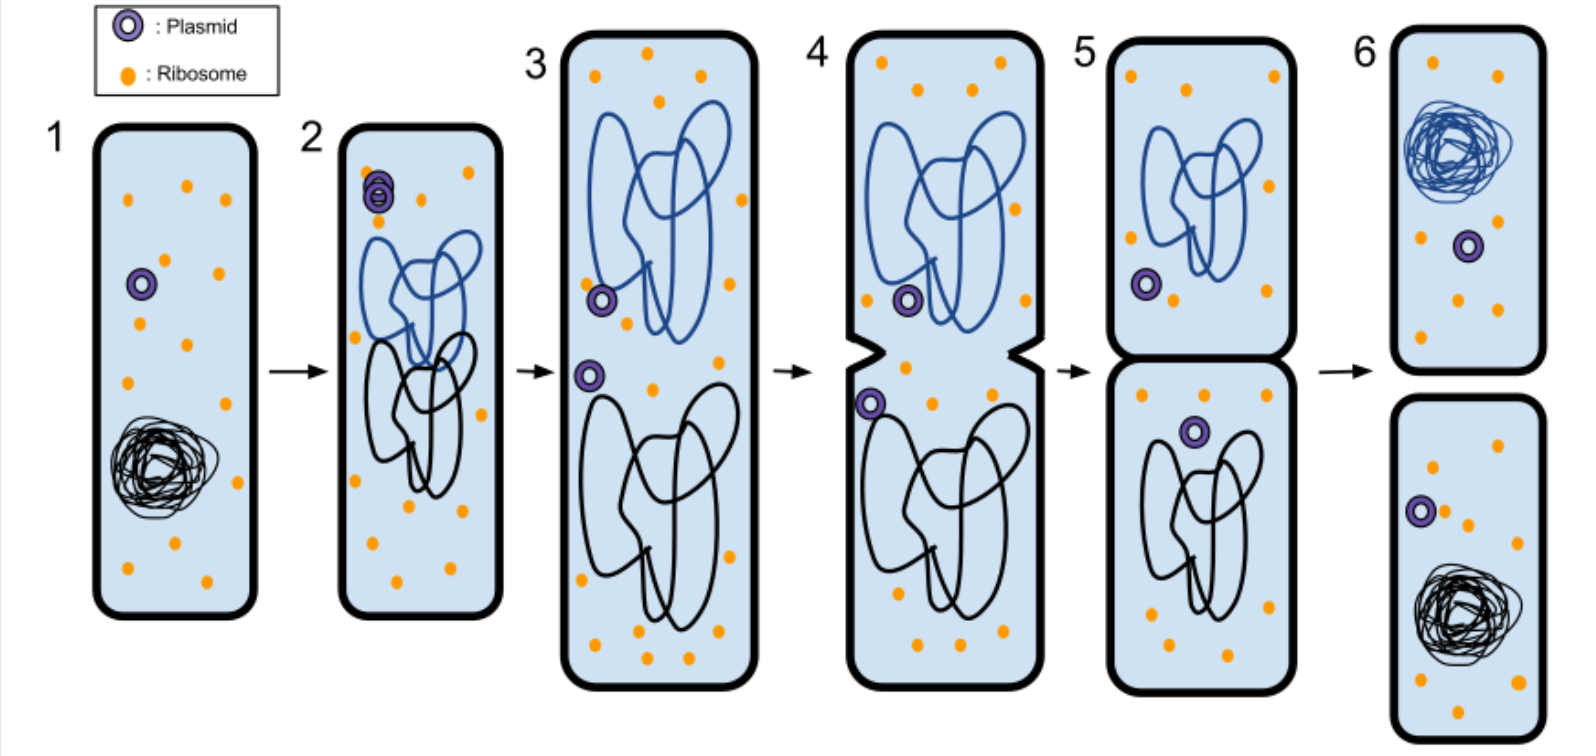
\includegraphics[width = 0.7 \linewidth]{6_deleniye.png}
    \caption{Деление бактериальной клетки: 1)  начальное состояние, 2) репликация ДНК, 3) сегрегация хромосом по клеткам, 4-5) образование перегородки между клетками, 6) финал, две клетки.}
    \label{fig:6_deleniye}
\end{figure}

\subsection{Репликация плазмид, мобильных элементов, фагов и вирусов.}

\begin{itemize}
    \item \textbf{Плазмиды} - небольшие кольцевые молекулы ДНК бактерий, физически обособленные от хромосом и способные к автономной репликации (то есть, вне стадии деления клетки). Они реплицируются по двум схемам: по типу катящегося колеса и по тета-типу (см. билет 3).
    
    \item \textbf{Мобильные генетические элементы} - куски генетического материала, которые могут путешествовать внутри генома и от одного организма к другому (буквально цепочки нуклеиновых кислот, отсоединяющиеся от хромосом в одном месте, диффундирующие, и встраивающиеся в другом)
    
    \item \textbf{Вирусы} - неклеточный инфекционный агент, который может воспроизводиться только внутри клеток. Вирус фактически представляет собой небольшую белковую машину и генетический материал.
    
    Вирус проникает в организм хозяина. Затем вирус прикрепляется к мембране клетки, специальными белками буравит клеточную мембрану и впускает внутрь свой генетический материал. Белки клетки начинают реплицировать генетический материал вируса и на его основе собирать белки, из которых получаются новые вирусы. 
    
    Когда все ресурсы клетки израсходованы, разможившиеся копии вируса разрывает клетку и высвобождаются для заражения новых клеток.
    
    \item \textbf{Бактериофаги} - вирусы, поражающие бактерии. К ним справедливо все то же самое, что изложено про вирусы.
    
\end{itemize}

\subsection{Особенности репликации в эукариотах. Теломеры и центромеры. Сегрегация хромосом.}

У эукариот молекулы ДНК линейны. Рассмотрим обычную (не половую, важно) клетку эукариот. 

\begin{itemize}
    \item Всю жизнь от рождения от материнской клетки дочерняя клетка живет с хромосомами. Хромосомы - длинные нити ДНК, на которых в некоторых местах еще сидят структурные белки. Число типов хромосом и число копий одного типа варьируется от вида к виду.
    
    \item Перед делением клетки ДНК хромосомы реплицируются и из одной материнской хромосомы получается две дочерние, называющиеся \textbf{сестринскими хроматидами} (см. рис. \ref{fig:6_chromatide}).
    
    \begin{figure}[h!]
        \centering
        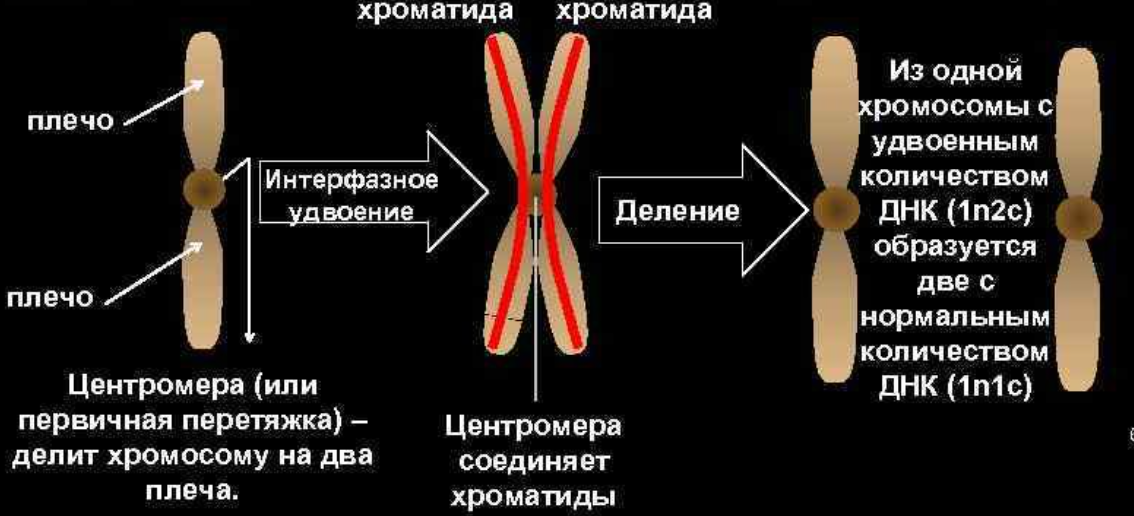
\includegraphics[width = 0.7 \linewidth]{6_chromatide.png}
        \caption{Хроматиды и хромосомы}
        \label{fig:6_chromatide}
    \end{figure}
    
    \item Хроматиды связаны белками в некоторой области. Эта область называется \textbf{центромера} (рис. \ref{fig:6_chromosome}).
    
    \item Концевые участки хромосом называются \textbf{теломеры}.
    
    \begin{figure}[h!]
        \centering
        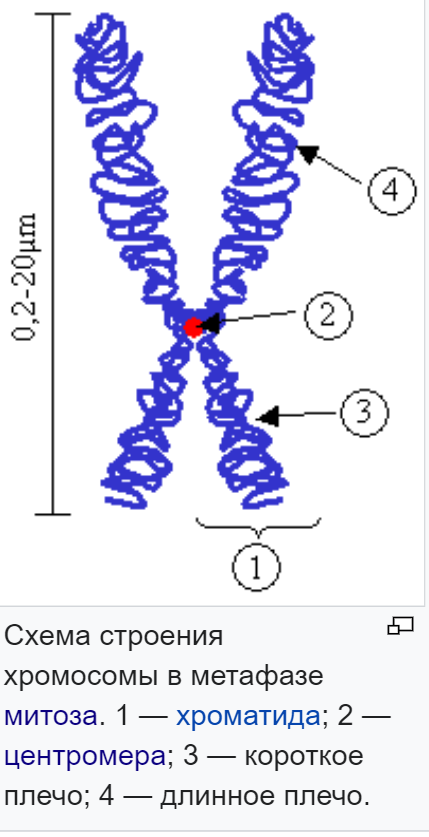
\includegraphics{6_chromosome.png}
        \caption{Хромосома, состоящая из двух хроматид}
        \label{fig:6_chromosome}
    \end{figure}
    
    \item В процессе клеточного деления происходит \textbf{сегрегация хромосом}. Каждой из двух дочерних клеток переходит одна из сестринских хроматид (см. подробнее митоз и мейоз). А ОКАЗАВШИСЬ В ДОЧЕРНЕЙ КЛЕТКЕ ХРОМАТИДЫ УЖЕ НАЗЫВАЮТСЯ СНОВА ХРОМОСОМАМИ НЕНАВИЖУ ОБОЗНАЧЕНИЯ БИОЛОГОВ
\end{itemize}

	
	\newpage
	
	\section{Мутагенез. Спонтанный мутагенез. Скорость мутагенеза.
Индуцированный мутагенез. Репарация димеров тимина с помощью фотолиазы и эксцизионной репарации.
Понятие сайт-специфического мутагенеза.}
	
\subsection{Мутагенез. Естественный мутагенез - Мутационная теория Де Фриза и Коржинского}

Мутагенез — процесс изменения в нуклеотидной последовательности ДНК, приводящий к мутациям. \\

Мутационная теория составляет одну из основ генетики. В ее основу были заложены идеи Де Фриза и Коржинского.

Основные положения мутационной теории Коржинского — Де Фриза можно свести к следующим пунктам (кратко):

\begin{enumerate}
	\item Мутации внезапны, как дискретные изменения признаков
	Новые формы устойчивы
	\item В отличие от наследственных изменений, мутации не образуют непрерывных рядов, не группируются вокруг какого-либо среднего типа. Они представляют собой качественные скачки изменений
	\item Мутации проявляются по-разному и могут быть как полезными, так и вредными
	\item Вероятность обнаружения мутаций зависит от числа исследуемых особей
	\item Сходные мутации могут возникать неоднократно
\end{enumerate}

\subsubsection{Механизмы мутагенеза}

Последовательность событий, приводящая к мутации выглядит следующим образом: происходит повреждение ДНК (если повреждение ДНК не было корректно репарировано, оно приведет к мутации); в случае, если повреждение произошло в незначащем фрагменте ДНК или если повреждение произошло в значащем фрагменте и, вследствие вырожденности генетического кода, не произошло нарушения, то мутации образуются, но их биологические последствия будут незначительными или могут не проявиться.

\subsection{Скорость мутагенеза}

Скорость мутагенеза - темп нуклеотидных замен. 

Как посчитать?\\

Один из самых простых способов - изучение родословных с целью подсчета вновь возникающих мутаций с четким фенотипическим эффектом и высокой пенетрантностью (то есть таких мутаций, которые меняют фенотип строго определенным образом и наверняка). Как правило, для этого используют мутации, вызывающие врожденные патологии, так как они  вызываются единичными мутациями.

\begin{figure}[H]
	\centering
	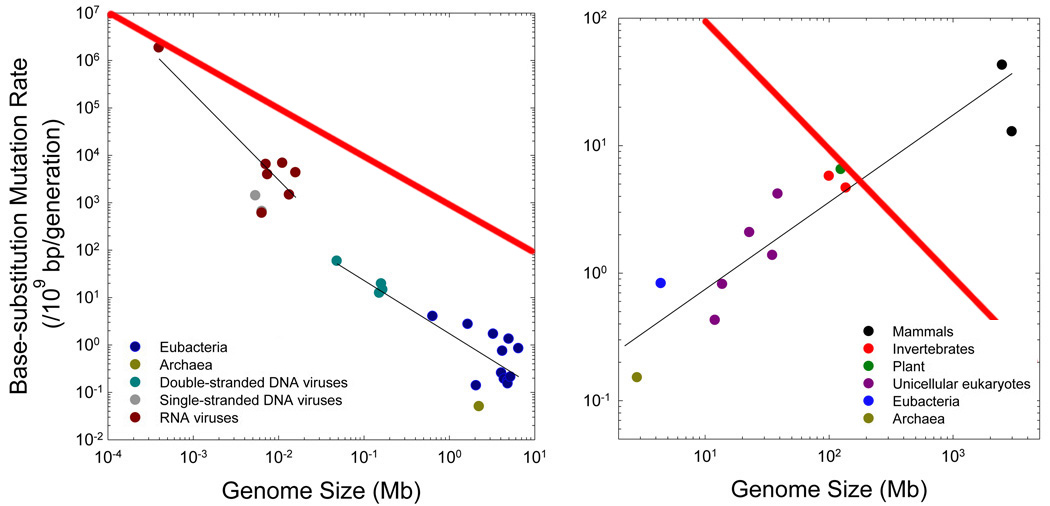
\includegraphics[width=0.7\linewidth]{7_mutation_pace}
	\caption{Скорость мутация, слева для вирусов и прокариот, справа для эукариот. По вертикали - темп нуклеотидных замен на миллиард пар оснований (bp - base-pair), по горизонтали - размер генома в миллионах оснований (Mb - Mega base). Вывод: для вирусов и прокариот чем сложнее организм, тем меньше скорость его мутагенеза, для эукариот - чем сложнее оргинзм, тем выше скорость его мутагенеза.}
	\label{7_mutation_pace}
\end{figure}
	
\subsection{Индуцированный мутагенез}

Искусственный мутагенез широко используют для изучения белков и улучшения их свойств. \\

\textbf{Ненаправленный мутагенез}

Методом ненаправленного мутагенеза в последовательность ДНК вносятся изменения с определённой вероятностью под воздействием мутагенных факторов — мутагенных веществ, ультрафиолета, радиации. \\

\textbf{Направленный мутагенез \ ПЦР - мутагенез}

Изменения в ДНК вносятся в заранее известный сайт. Для этого синтезируют короткие одноцепочечные молекулы ДНК (праймеры), комплементарные целевой ДНК за исключением места мутации. \\

\textbf{Вставной мутагенез}

Cоздание мутаций ДНК путем добавления одной или более пар оснований. \\

\subsection{Понятие сайт-специфического мутагенеза}

Сайт-направленный мутагенез является методом молекулярной биологии, который используется, чтобы создать конкретные и преднамеренные изменения в последовательности ДНК, гена и продуктов генов.

\begin{figure}[H]
	\centering
	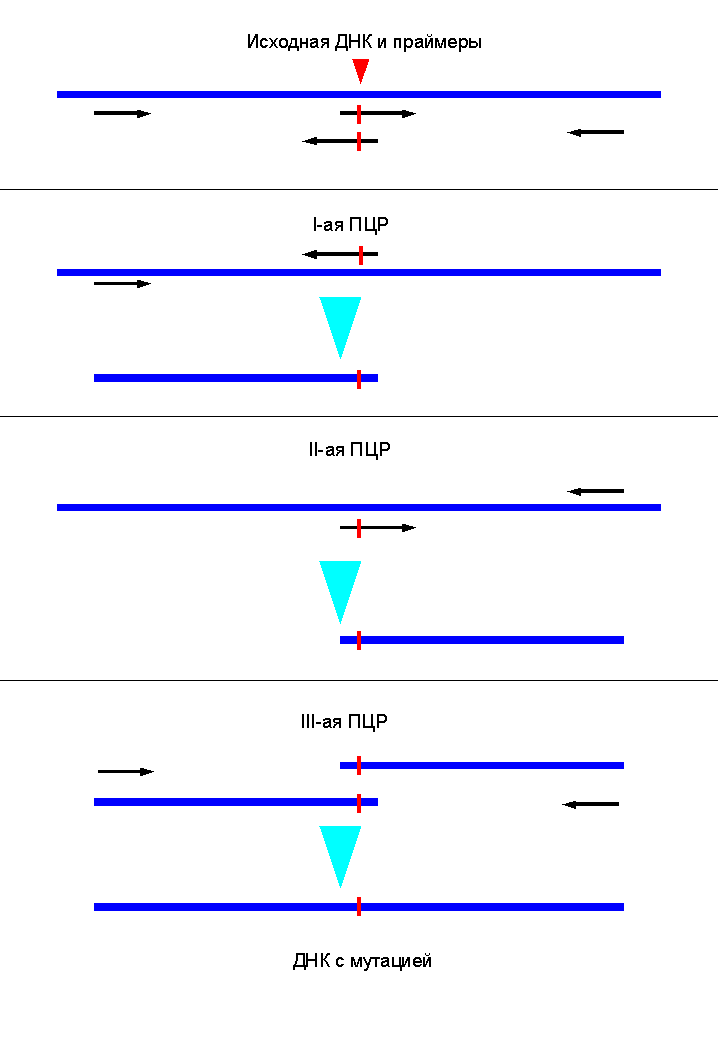
\includegraphics[width=0.7\linewidth]{7_site_mutagenesis}
	\caption{Сайт-направленный мутагенез. Синтезируют пару праймеров, несущих мутацию, и пару праймеров, комплементарных концам нужного фрагмента ДНК. В ходе первых двух реакций образуются фрагменты ДНК с мутацией, которые объединяют в третьей реакции. Полученный фрагмент вставляют в нужную генно-инженерную конструкцию.}
	\label{7_site_mutagenesis}
\end{figure}

\subsection{Репарация димеров тимина с помощью фотолиазы и эксцизионной репарации}

Пиримидиновый димер — дефект ДНК, возникающий в результате образования ковалентной связи между двумя соседними пиримидиновыми основаниями (тимином или цитозином) под действием ультрафиолетовых лучей. Ультрафиолетовые лучи вызывают разрыв двойной связи и образование в этом месте ковалентной связи между двумя нуклеотидами. Образование димера приводит к нарушению транскрипции ДНК на данном участке и возникновению мутаций.

\begin{figure}[H]
	\centering
	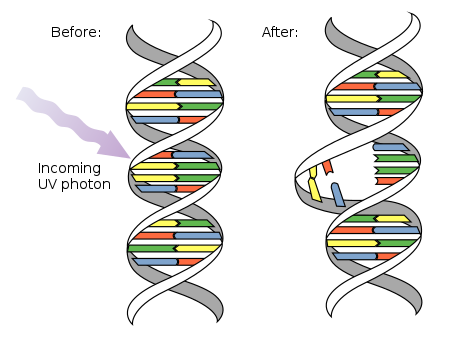
\includegraphics[width=0.7\linewidth]{7_dna_lesion}
	\caption{Дефект ДНК - димер тимина}
	\label{7_dna_lesion}
\end{figure}
	
\begin{figure}[H]
	\centering
	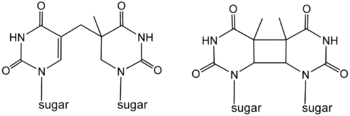
\includegraphics[width=0.7\linewidth]{7_timin_dimer}
	\caption{То, что образуется в результате дефекта. Слева: 6,4-фотопродукт. Справа: циклобутановый димер}
	\label{7_timin_dimer}
\end{figure}
	
\subsubsection{Репарация ДНК}

\textbf{ДНК-фотолиаза}

Один из способов удаления пиримидиновых димеров состоит в ферментативном превращении их в мономеры при освещении видимым светом в диапазоне длин волн 300—600 нм. ДНК-фотолиаза образует стабильный комплекс с пиримидиновым димером и, используя энергию поглощённого им света, разрушает димер без разрыва цепей ДНК. \\

\textbf{Эксцизионная репарация нуклеотидов}

Подразумевает удаление повреждённых азотистых оснований из ДНК и последующее восстановление нормальной структуры молекулы по комплементарной цепи. Ферментативная система удаляет короткую однонитевую последовательность двунитевой ДНК, содержащей поврежденные основания, и замещает их путём синтеза последовательности, комплементарной оставшейся нити. \\

	
	\newpage
	
		\section{Гомологичная рекомбинация. Модель Холлидея.
		Гены рекомбинации (recA, ssb, ruvABC). RecA и SOS-ответ.
		Сайт-специфическая рекомбинация. 
		Рекомбинация в эукариотах. Кроссинговер.}
	
\textbf{Рекомбинация} -- возникновение новых последовательностей ДНК за счёт разрывов и пересоединений уже имеющихся молекул.
\textbf{Синаптический комплекс} -- комплекс из двух ДНК с перекрещивающимися цепями
\subsection{Гомологичная (общая) рекомбинация, модель Холидея}
Обмен участками между гомологичными (практически одинаковыми по последовательностям)  молекулам ДНК. За счёт гомологичной рекомбинации не создаются новые последовательности, а перемешиваются имеющиеяс похожие варианты одной и той же последовательности.

Характеризуется следующими стадиями (Рис \ref{pic:8_holi})
\begin{enumerate}
\item Делаются два разреза в одинаковых положениях цепи
\item Одна цепь высвобождается, за счёт RecA ищет гомологичный кусок 
\item Образуется D-loop, засчёт того, что смещённая цепь вытеснила кусок другой
\item D-loop рвётся и образуется структура Холидея
\end{enumerate}
  
 Крест Холидея может двигаться при этом в обе стороны рекомбинирующих молекул, при этом сами молекулы вращаются вокруг своей оси, а гетеродуплексный (из разных кусков) участок удлиняется или укорачивается. 
 
 При этом цепи ДНК в гетеродуплексе не обязательно комплементарны и в результате рекомбинации могут образовывать разный результат. Если неспаренные основания не репарируются, то каждая цепь даст такой же дуплекс, как у родительской ДНК, если репарация происходит, то часть одной цепи станет совпадать со второй цепью.
 
 Куски при этом можно по разному резать (см \ref{pic:8_holi} д, е )
 
 Таких структур может быть несколько, получаются из-за чего более сложные объекты
 \begin{figure}[H]
 	\centering{
 	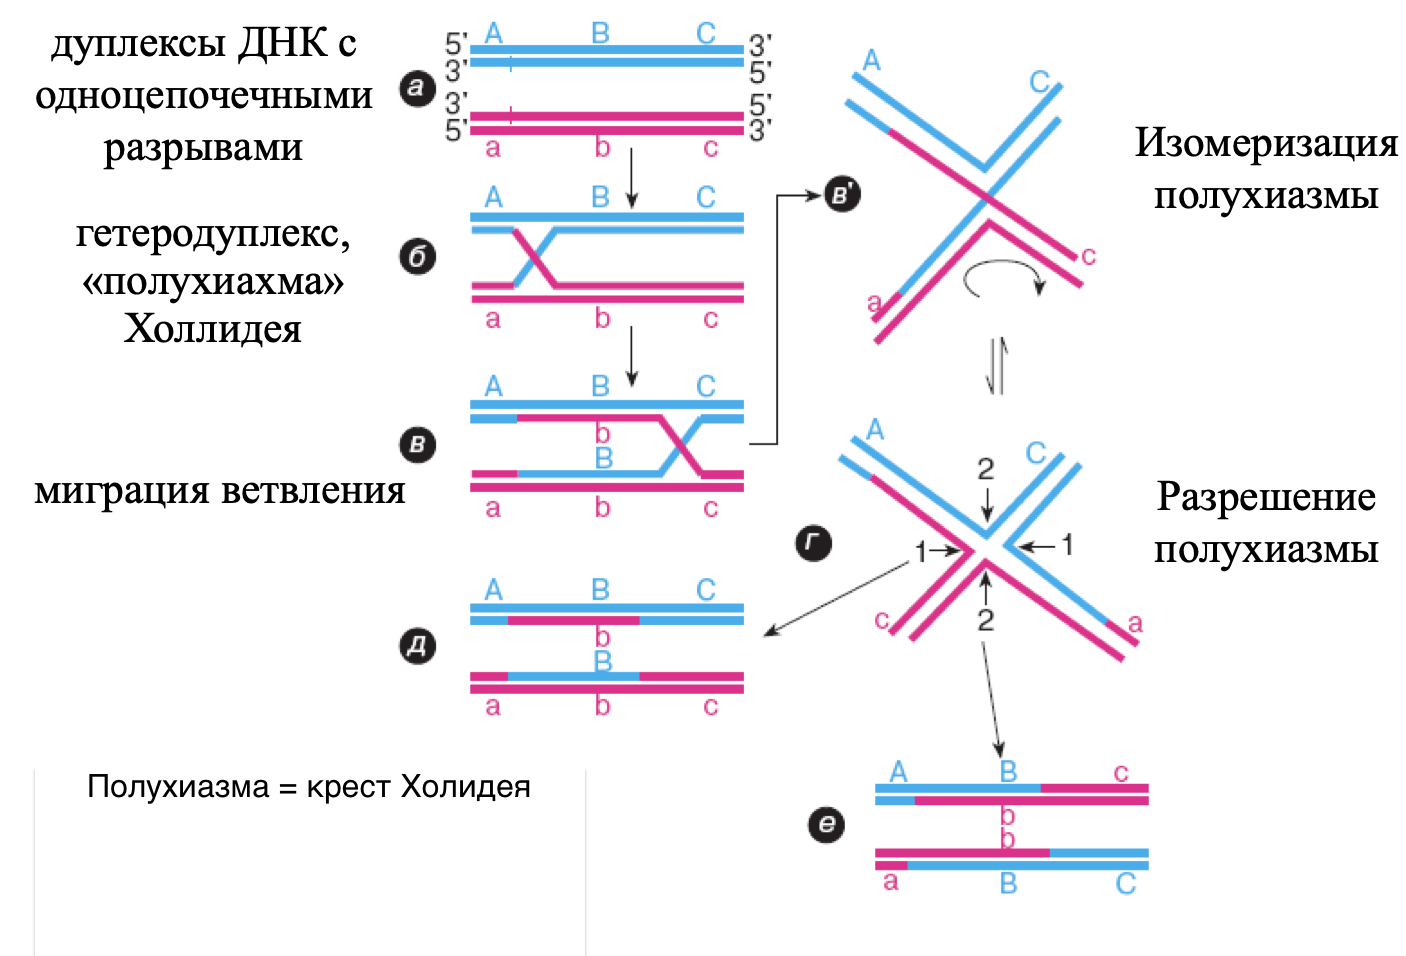
\includegraphics[scale=0.5]{8_holi.png}
 	\caption{Основные стадии общей рекомбинации}
 	\label{pic:8_holi}}
 \end{figure}
 	
\subsection{Гены рекомбинации}
\paragraph{RecA}  -- консервативный белок, который есть и у прокариотов, и у эукариотов, хотя при этом по нему можно получить мутацию. Важен для эволюции, поэтому как доп функция у бактерий -- запускает SOS-ответ. 

Умеет связываться с одноцепочечной ДНК (нарастает в сторону 3' конца) и искать гомологию, а потом переносить одноцепочечный фрагмент на двухцепочечный, который после расплетает, после чего формируется гетеродуплекс. Умеет связываться с двуцепочечной ДНК, но реже. 
\paragraph{SSB} -- Связываются с одноцепочечной ДНК и не дают ей связаться в двойную цепь, что препятствовало бы рекомбинации.Также ускоряет среднюю скорость синтеза ДНК бактериальными и архейными полимеразами..
\paragraph{ruvABC} $\ $\newline



 ruvA -- связывается со всей структурой Холидея и стабилизирует её
 
 ruvB -- белок, который вращает ДНК для продвижения креста. Тесно связывается с ruvA, поэтому вращение ДНК происходит ещё и относительно ruvA. 
 
 ruvC -- белок, который разрезает структуру Холидея симметрично с обеих сторон. У ruvC есть некоторая предпочтительная последовательность, поэтому разрезание происходит только на специфическом сайте. 
 	\begin{figure}[H]
 	\centering
 	\subfigure[a][ruvAB]{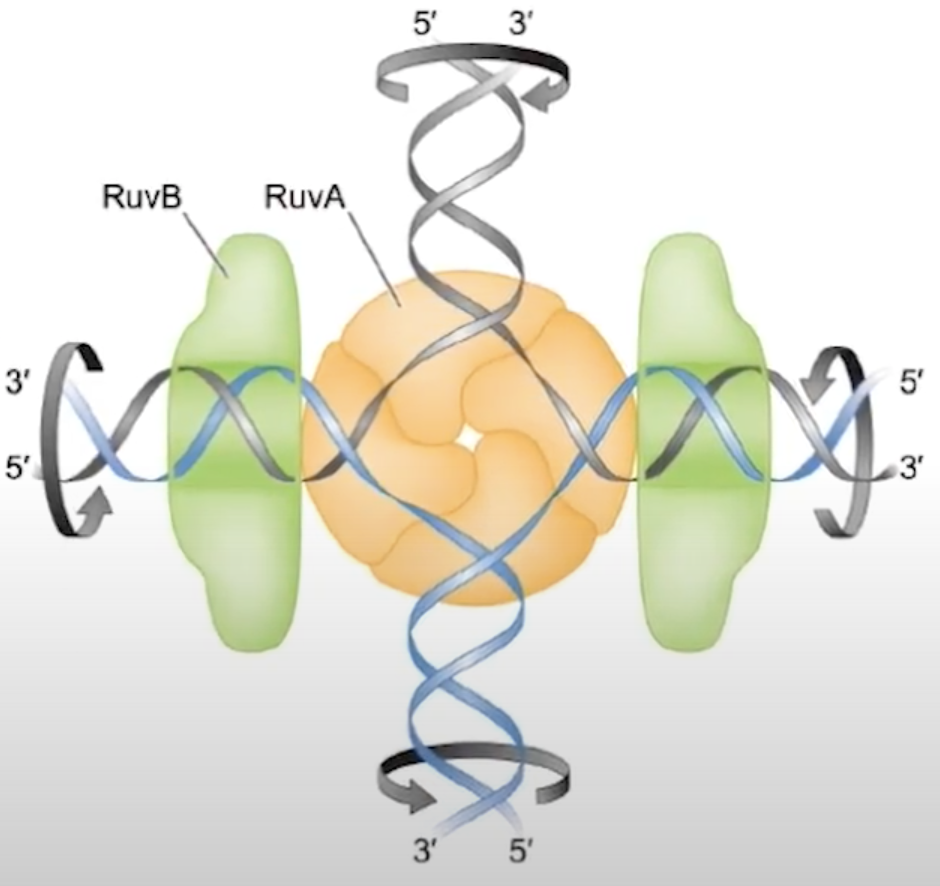
\includegraphics[scale=0.5]{8_ruvAB.png}}
 	\qquad
 	\subfigure[b][ruvC]{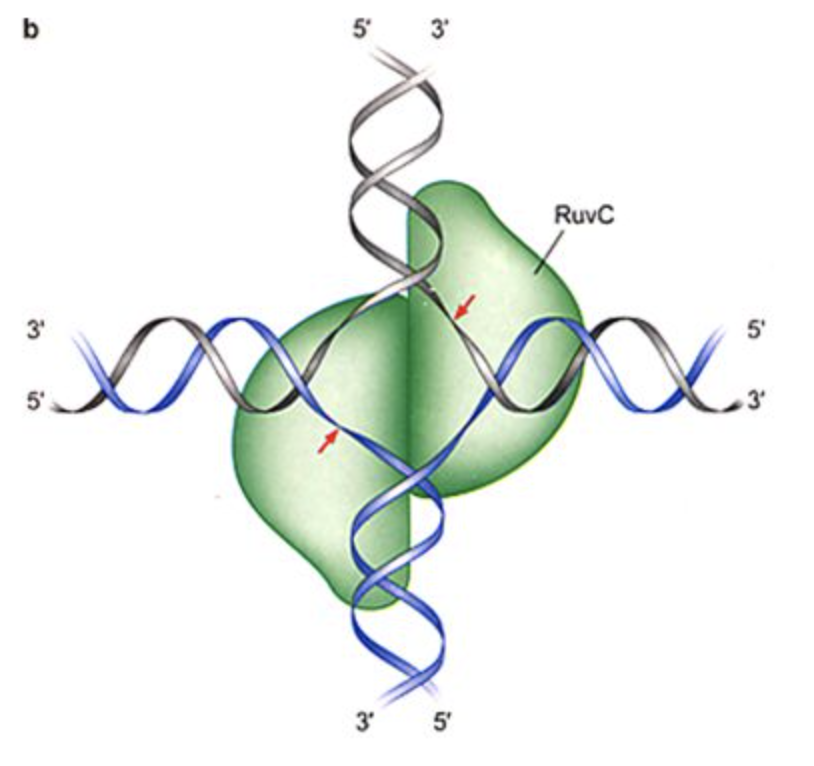
\includegraphics[scale=0.5]{8_ruvC.png}}
 \end{figure}
 	
\subsection{SOS-ответ и recA}

При малом количестве повреждений увеличивается количество uvrАBCD. 

При большом блокируется деление клеток и тем самым индуцируется синтез RecA, который нужен для рекомбинационной репарации. В активной конформации RecA стимулирует деградацию LexA (репрессора, в том числе себя и RecA, umuCD (ДНК полимераза-5), uvrABCD), после чего транскрибируются ген uvrB, продукты которого транскрибируются в эксцезионной репарации. 

Также RecA может umuCD откусывается RecA, оставляя umuC'D'

При ещё большем числе повреждений активируются umuCD, продукты которых позволяют полимеразе копировать нарушенный участок матрицы (вероятно позволяют им удлинять затравку), из-за чего больше мутаций. 
\subsection{Сайт-специфическая рекомбинация}
Не требует протяжённых участков гомологии, но требуются строго определённые последовательности ДНК и специальный ферментативный аппарат.

Происходит обычно при встраивании бактериофага в геном бактерии. 

\paragraph{Общая схема} Последовательность, которая,  способна к рекомбинации окружена специальными сайтами, которые узнаются рекомбиназой, а потом, например, меняют положение последовательности в последовательности. В зависимости от расположения сайтов рекомбинации получаются разные результаты, так как каждые сайты рекомбинации асимметричны.

Сам сайт при этом выглядит как асимметричный кусок посередине и два куска, которые одинаково читаются при прочтении с разных сторон (палиндромы). Каждые куски-палиндромы связываются с рекомбиназой, после чего вносятся разрывы в ДНК. (см Рис. \ref{pic:8_ssrec}). Сначала отрывается одна цепь, потом соединяется, формируя структуру, похожую на Холидеевский крест, а потом вторая нитка разрывается и перестраивается. 
 \begin{figure}[H]
	\centering{
		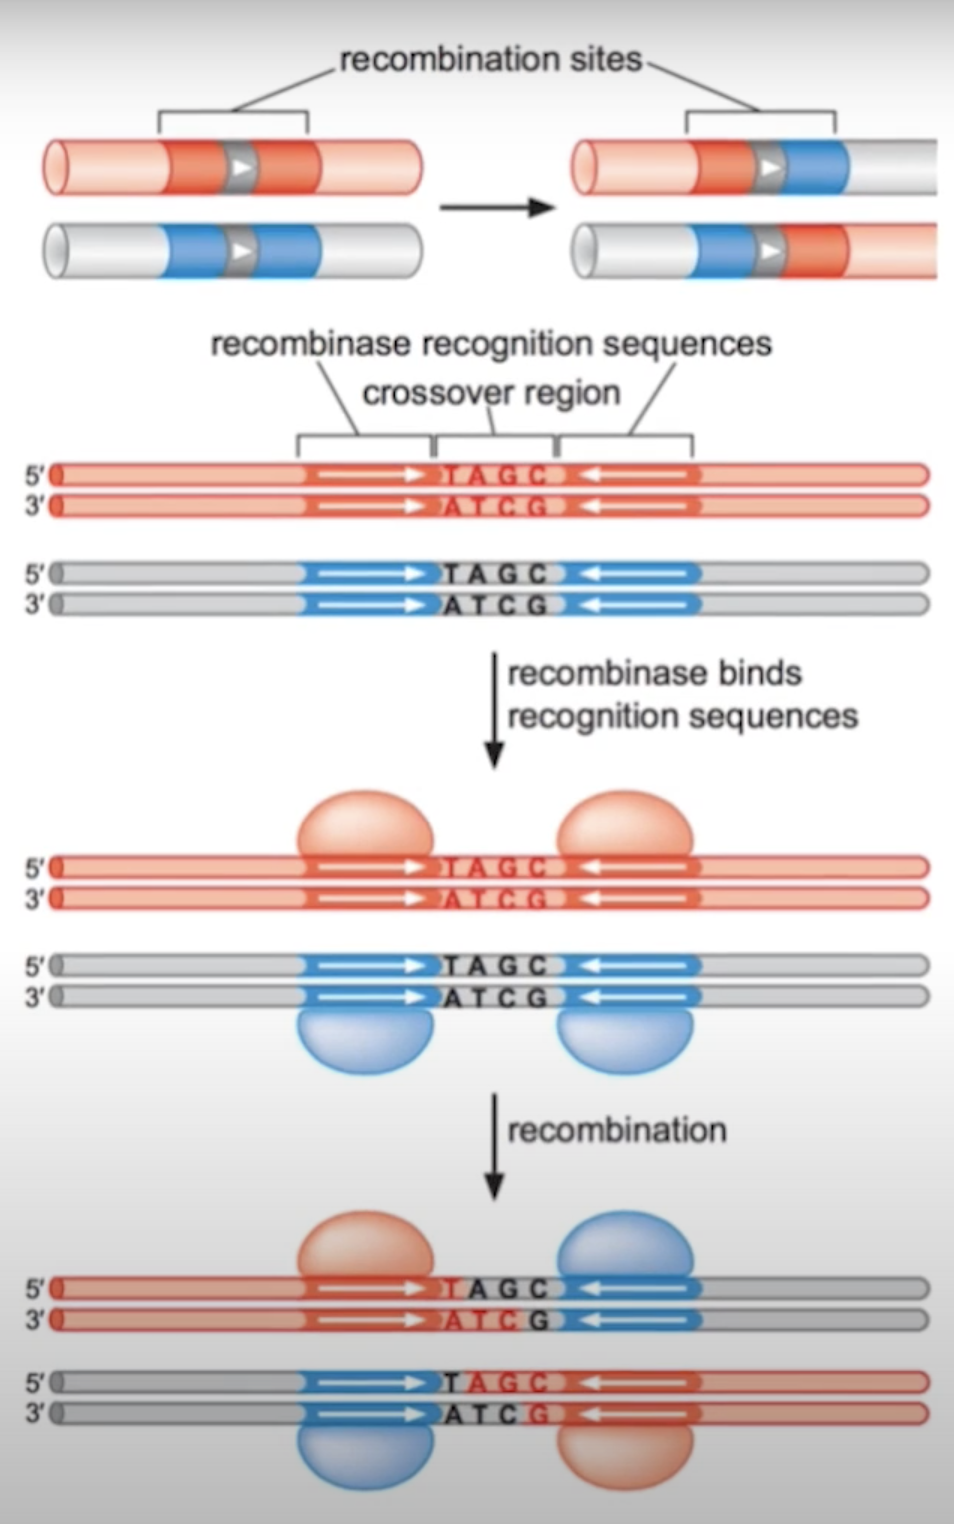
\includegraphics[scale=0.5]{8_ssrec.png}
		\caption{Сайт-специфическая рекомбинация в общем виде}
		\label{pic:8_ssrec}}
\end{figure}
\subsubsection{Транспозиция}
\textit{Я не верю в адекватность пахома, так что пусть это тут тоже будет на всякий}

Бывает нерепликативная и репликативная. Транспозоны (переезжающие куски) окружены похожими сайтами, как у сайт-специфической рекомбинации. 

\paragraph{ДНК транспозоны} Ген, необходимый для транспозиции (транспозон) окружён инвертированными концами. Дальше концов идут инвертированные концы (как палиндромы)

Инвертированные концевые повторы связываются, после них вносятся разрывы, а далее 3' концы встраиваются в ДНК, в которую будут вставляться транспозоны
 \begin{figure}[H]
	\centering{
		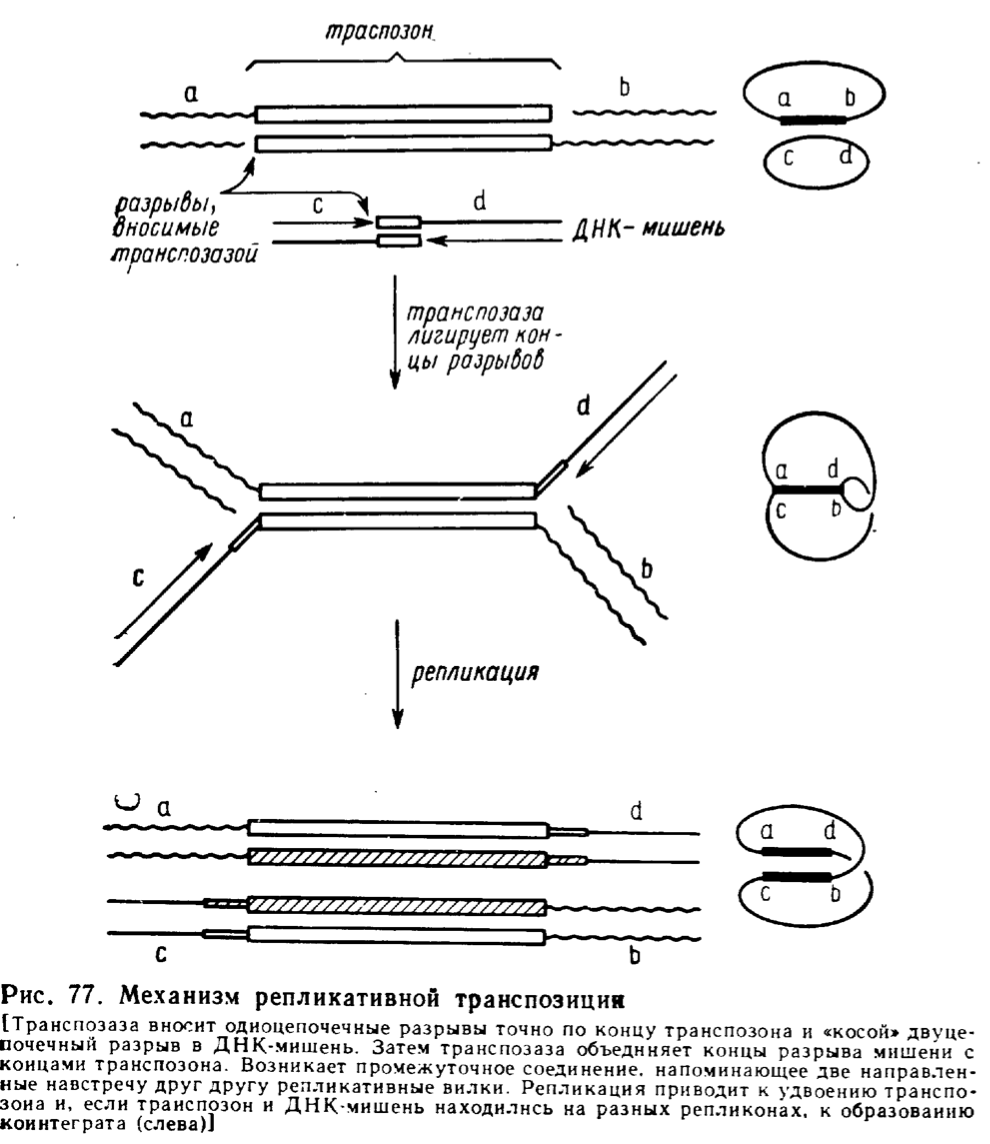
\includegraphics[scale=0.5]{8_transp.png}
		\caption{Сайт-специфическая рекомбинация в общем виде}
		\label{pic:8_transp}}
\end{figure}
\paragraph{Вирус-подобные ретропозоны} Длинные концевые повторы, потом посередине интеграза (встраивает в геном) и обратная транскриптаза. 

Сначала в ретропозоне в крайнем промоторе транскрибируется полная копия генома, потом обратной транскрипцией РНК переходит в ДНК, в котором образуются повторы, которые так же, ккак и в случае транспозонов встравиваются в днк
\section{Рекомбинация в эукариотах}
\paragraph{Мейотическая}
Перед первым делением мейоза хроматиды удерживаются вместе, но из-за кроссинговера гомологичные хромосомы тоже оказываются связаны (для правильной ориентации). Как правило рекомибанция начинается с одноцепочечного разрыва и происходит по модели Мезелсона Рэддинга (Рис \ref{pic:8_mes_red})
 \begin{figure}[H]
	\centering{
		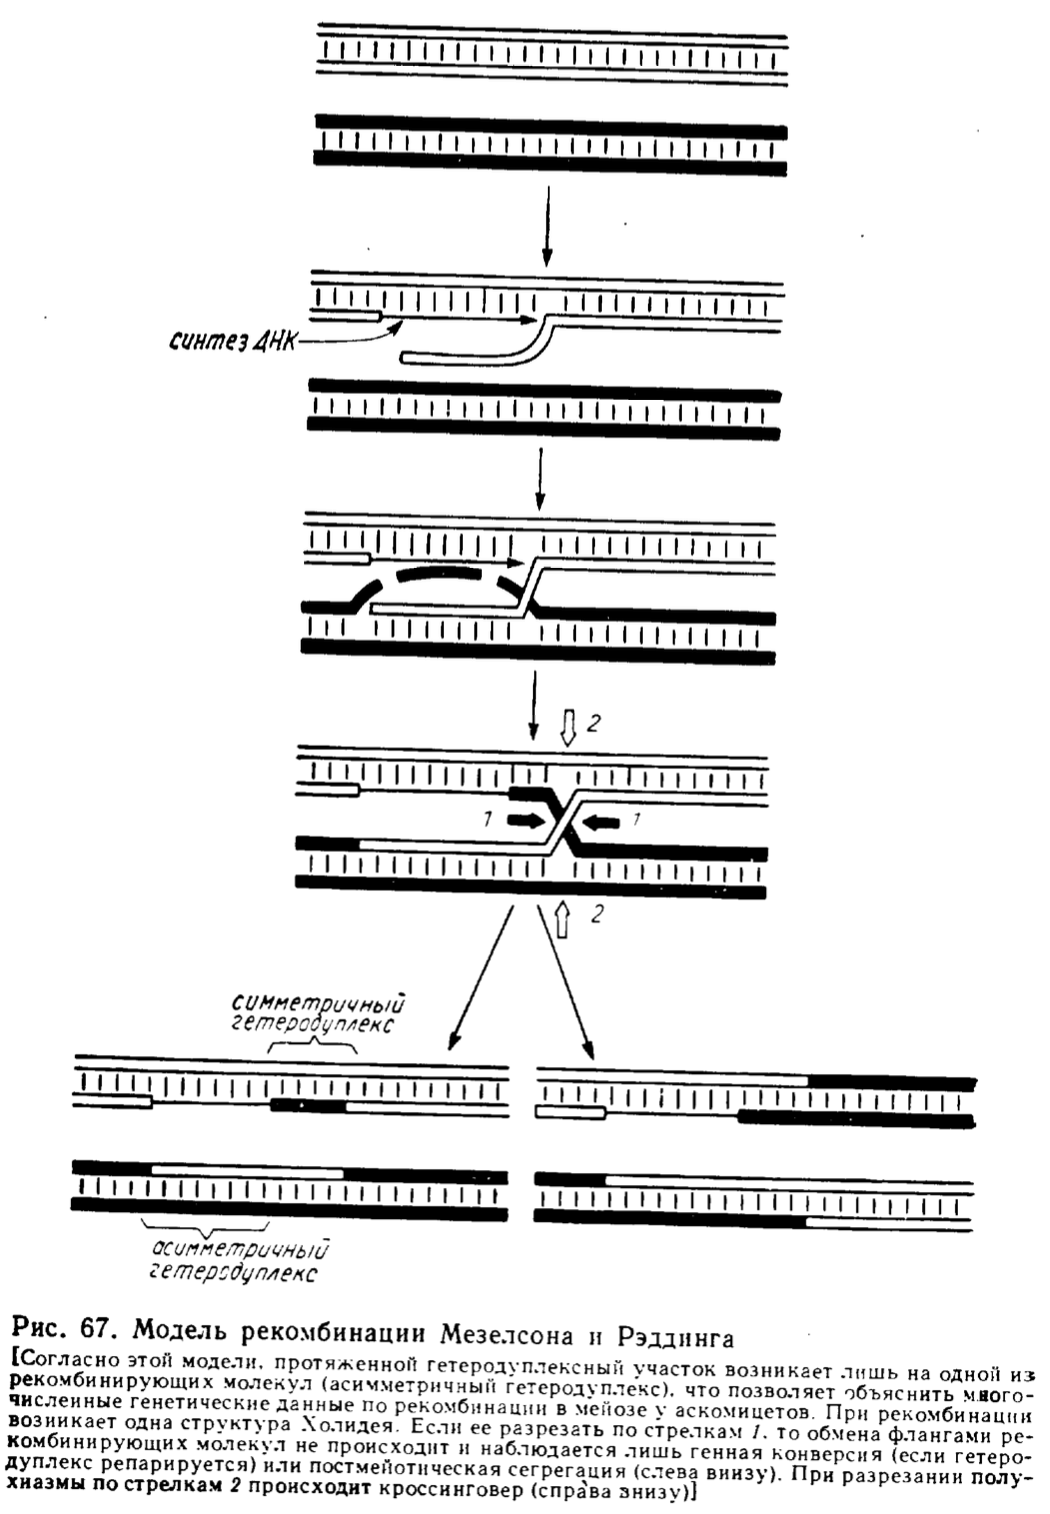
\includegraphics[scale=0.7]{8_mes_red.png}
		\caption{Мейотическая рекомбинация. Хиазм -- область связывания засчёт кроссинговера, похожая на Холидеевский крест}
		\label{pic:8_mes_red}}
\end{figure}
\paragraph{Митотическая}
Рекомбинация происходит между гомологичными генами соматических клеток многоклеточных или при вегетативном росте одноклеточных. Большинство случаев рекомбинации связаны с репарацией. Притом стимулирует рекомбинацию не только разрыв, но и двуцепочечная брешь (Рис. \ref{pic:8_eu_rec}). Характерно образование двух холидеевский крестов. Брешь при этом застраивается по образу и подобию неповреждённой молекулы. Центральную роль снова играет белок, похожий на RecA.
 \begin{figure}[H]
	\centering{
		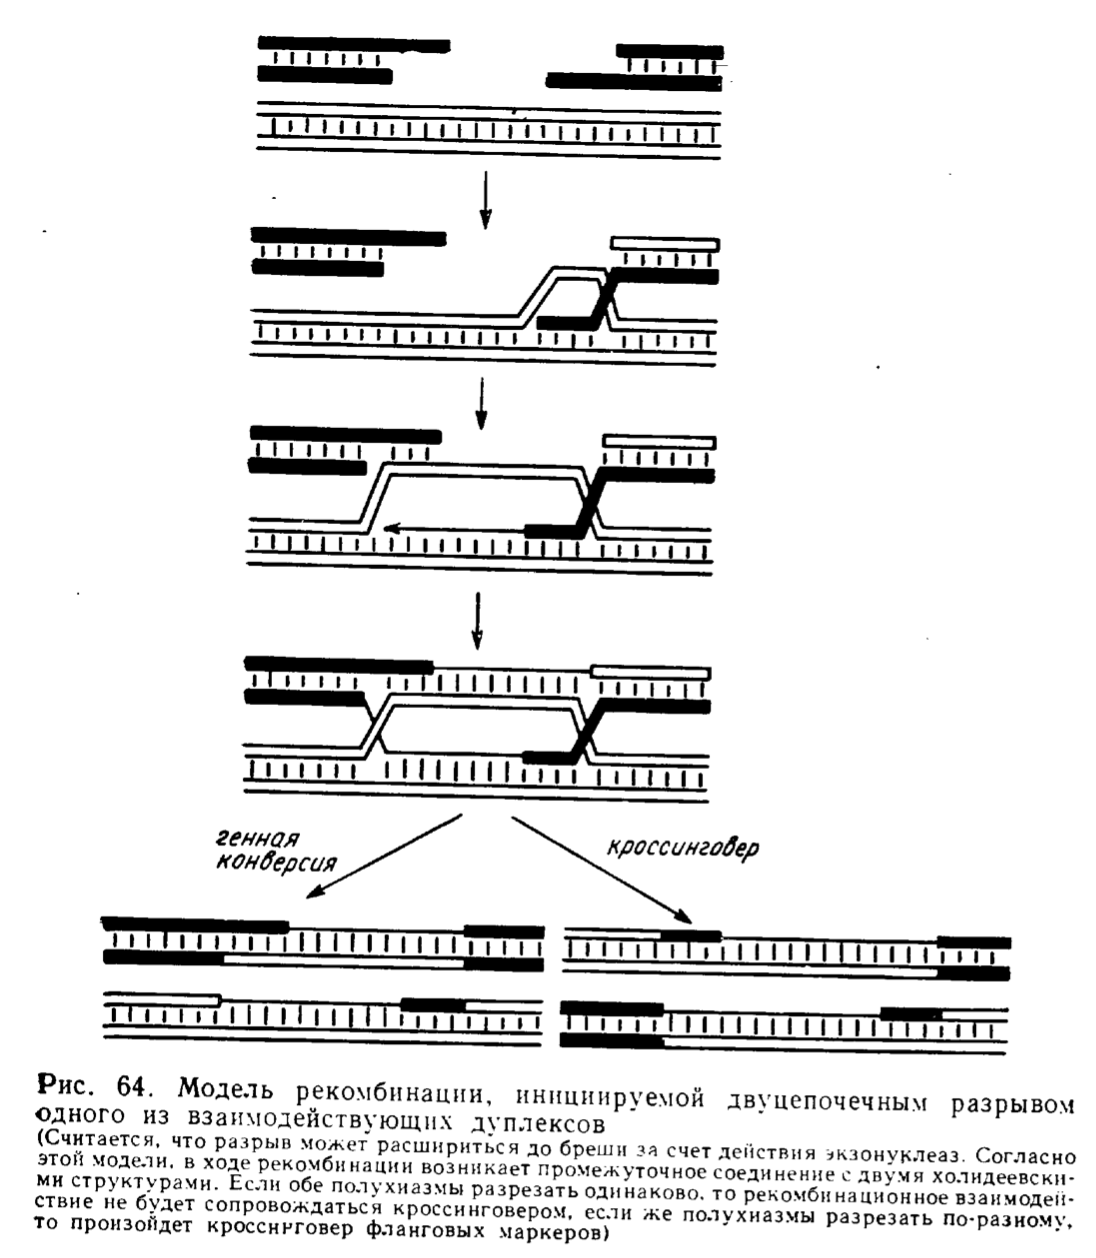
\includegraphics[scale=0.7]{8_eurec.png}
		\caption{Митотическая рекомбинация}
		\label{pic:8_eu_rec}}
\end{figure}
\paragraph{Кроссинговер} -- рекомбинационный обмена участками гомологичных хромосом во время конъюгации (их спаривание) в профазе первого деления мейоза. (Разрыв и переклеивание родительских хромосом).
	
	\newpage
	
	\section{Промоторы прокариот и регуляторные элементы. Лактозный оперон. Аттенюация на примере 
триптофанового оперона. 
Промоторы эукариот. Энхансеры и сайленсеры. 
Альтернативный сплайсинг.}

\subsection{Промотор}

\textbf{Промотор} - последовательность нуклеотидов ДНК, узнаваемая РНК-полимеразой как стартовая площадка для начала транскрипции. 

По активности промоторы делят на:
\begin{itemize}
    \item конститутивные (постоянный уровень транскрипции);
    \item индуцибельные (транскрипция зависит от условий в клетке, например от присутствия определенных веществ или наличия теплового шока).
\end{itemize}

Активация промотора определяется присутствием набора транскрипционных факторов.

\subsection{Промоторы прокариот и регуляторные элементы}
У прокариот обычно имеется общий промотр сразу для нескольких генов (ген - последовательность ДНК с информацией о том, как строить белок). Эти несколько генов называют \textbf{опероном}, они всегда транскрибируются вместе. 

\textbf{Регуляторные элементы} - это белки, регулирующие активацию промоторов. Фактически, это белки, помогающие РНК-полимеразе связаться с конкретным опероном. Регуляторные элементы реагируют на внешние раздражители по изменениям концентрации различных веществ в клетке и запускают/гасят синтез РНК тех белков, которые сейчас нужны/не нужны для выживания.

\subsection{Лактозный оперон}
В норме бактерия кушает глюкозу (сахар), и не способна кушать лактозу (дисахарид, состоящий из двух сахаров, глюкозы и галактозы (см. рис. \ref{fig:9_lactose})). Синтезировать белки, которые позволяют кушать лактозу, в присутствии глюкозы невыгодно.

Но бывают ситуации, когда в среде вокруг бактерии нет глюкозы, но есть лактоза. Тогда активизируется \textbf{лактозный оперон} и начинает транскрибироваться группа генов, кодирующая белки, позволяющие кушать лактозу. 

\begin{figure}[H]
    \centering
    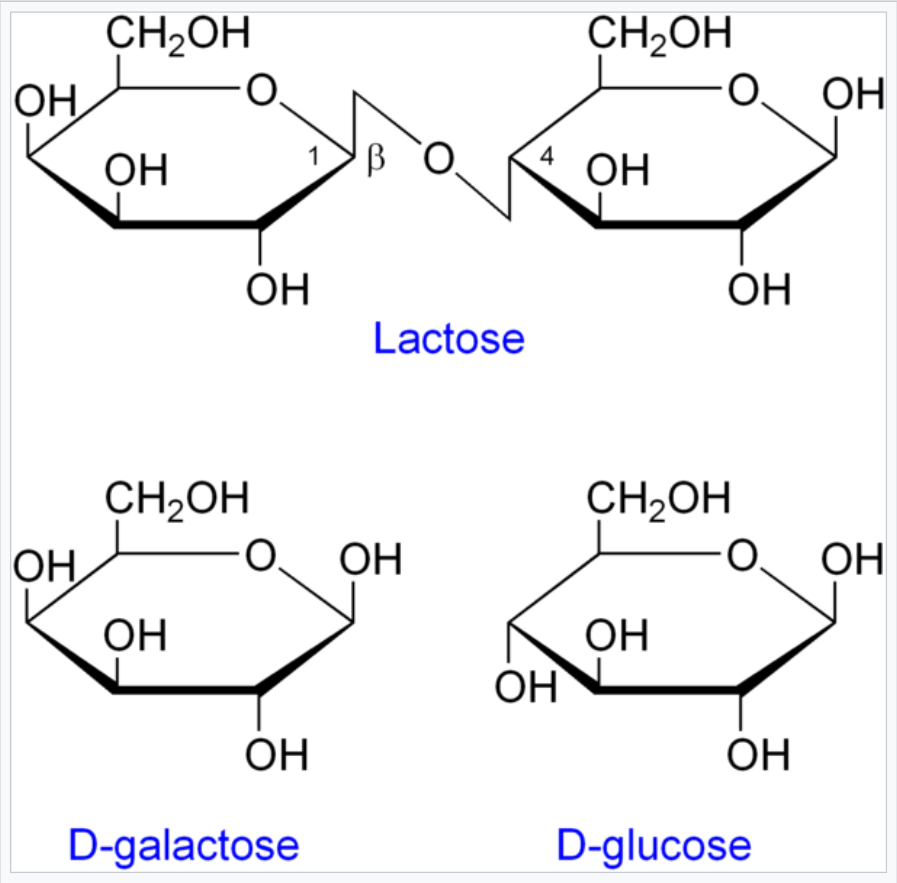
\includegraphics[width = 0.6 \linewidth]{9_lactose.png}
    \caption{Разница между глюкозой и лактозой (греческие буквы указывают конкретные изомеры феществ, то есть геометрическое строение).}
    \label{fig:9_lactose}
\end{figure}

Рассмотрим подробнее молекулярный механизм активации лактозного оперона. 

\begin{itemize}
    \item Лактозный оперон состоит из трех генов (см. рис. \ref{fig:9_glucose_on}-\ref{fig:9_lactose_on}): 
    
    a) ген lacZ, кодирует фермент \(\beta\)-галактозидазу, расщепляющий дисахарид лактозу на глюкозу и галактозу;
    
    б) ген lacY, кодирует фермент  \(\beta\)-галактозидпермеазу, протаскивающий лактозу из внешней среду в клетку через клеточную мембрану;
    
    в) третий ген, роль которого не ясна, поэтому нахуй его называть.
    
    \item Белок-репрессор в нормальных условиях сидит на операторном участке ДНК и мешает транскрипции (см. те же картинки).
    
    \item При повышенной концентрации лактозы репрессор связывается с лактозой, меняет свою форму и не может больше удерживаться на ДНК.
    
    \item Глюкоза подавляет синтез вещества цАМФ (циклическая форма аденазин-монофосфата). В отсутствии глюкозы это вещество синтезируется и дает сигнал белку CAP о клеточном голоде.
    
    \item Белок CAP садится на промотор лактозного оперона и облегчает его связывание с РНК-полимеразой.
    
    \item Запускается синтез белков, расщепляющих лактозу.
    
    
\end{itemize}

\begin{minipage}{.49\textwidth}
    \begin{figure}[H]
        \centering
        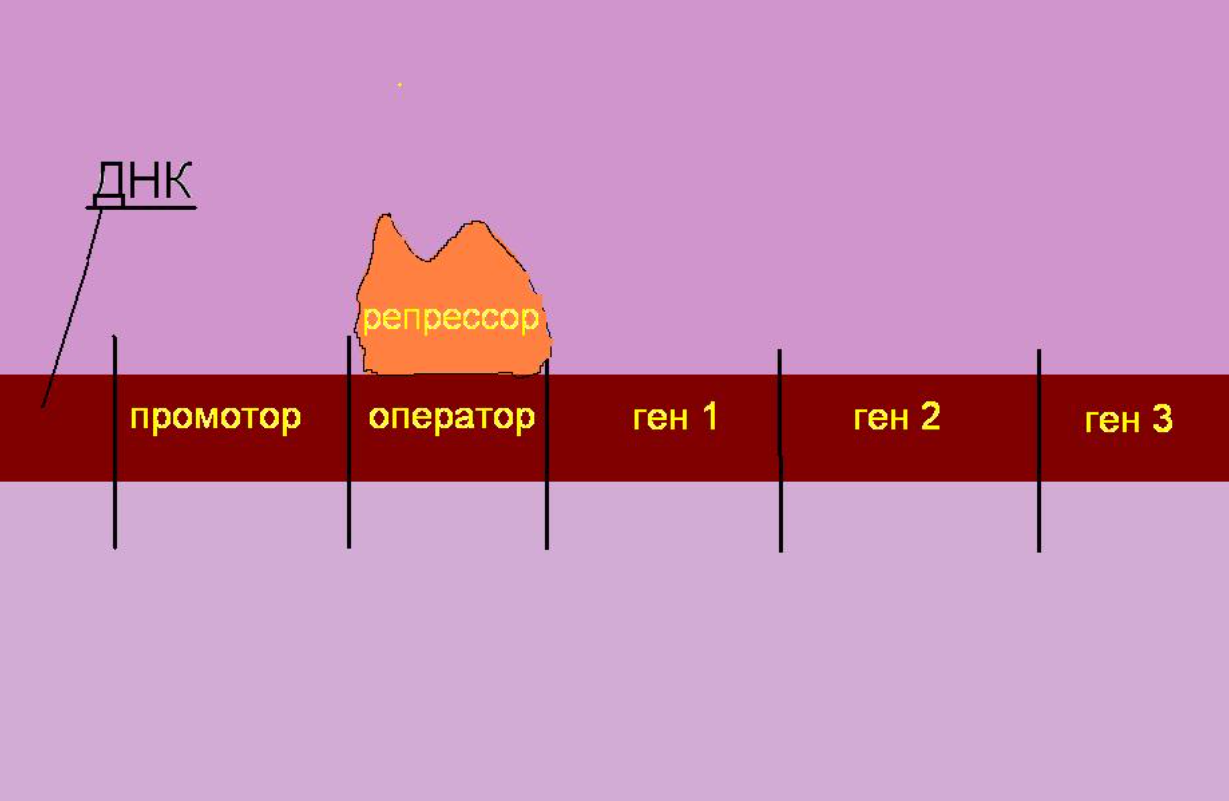
\includegraphics[width = 0.9 \linewidth]{9_glucose_on.png}
        \label{fig:9_glucose_on}
        \caption{Нет лактозы, есть глюкоза. Белок-репрессор подавляет транскрипцию генов поедания лактозы, сидя на операторе (участок оператора так и называется потому, что оперирует транскрипцией).}
    \end{figure}
\end{minipage}
\begin{minipage}{.49\textwidth}
   \begin{figure}[H]
        \centering
        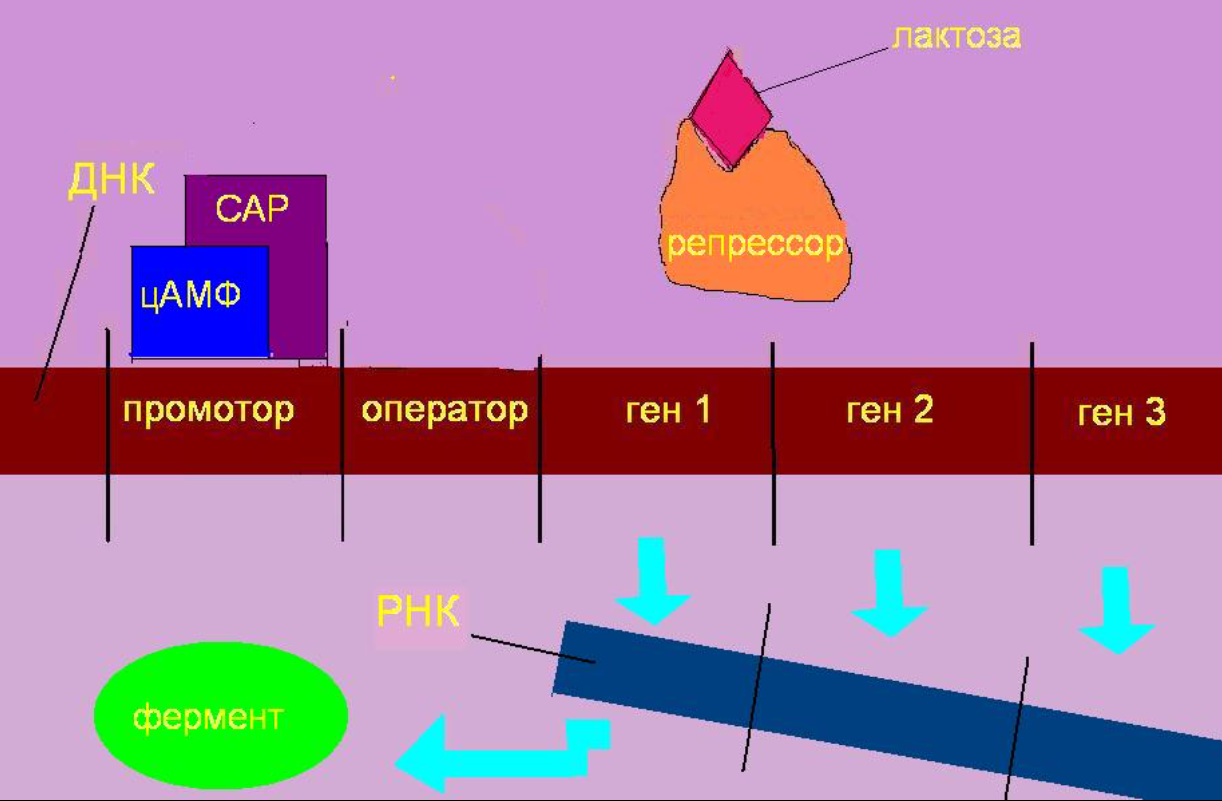
\includegraphics[width = 0.9 \linewidth]{9_lactose_on.png}
        \label{fig:9_lactose_on}
        \caption{Нет глюкозы, есть лактоза. Лактоза связывается с белком-репрессором, белок-репрессор меняет свою форму и больше не держится на ДНК. Приходят белок CAP c цАМФ и упрощают связывание РНК-полимеразы с промотором лактозного оперона.}
    \end{figure}
\end{minipage}

\subsection{Аттенюация на примере 
триптофанового оперона}

\textbf{Триптофановый оперон} — оперон, содержащий гены ферментов, задействованных в биосинтезе аминокислоты триптофан. Далее будем называть его trp-оперон (от англ. tryptophan). 

\textbf{Аттенюация} - способ регулирования транскрипции генов, характерный \textbf{только} для прокариот, у эукариот он не возможен. 

Суть в следующем. У прокариот процессы трансляции и транскрипции происходят одновременно. То есть РНК-полимераза еще не закончила делать РНК по матрице ДНК, а рибосома уже садится на недоделанную РНК и начинает транслировать с нее белки. В случае \textbf{аттенюации} происходит так, что \textbf{процесс трансляции прерывает процесс транскрипции}.

Ниже расписано, как аттенюация происходит на молекулярном уровне в регуляции триптофанового оперона (см. рис. \ref{fig:9_tryptophan}).

\begin{itemize}
    \item В trp-промоторе первая транскрибируемая область называется trpL (от leader), по ней затем рибомосомой транслируется leader peptide (маленький белок).
    
    \item В РНК, построенном по trpL выделяются 4 области - 1, 2, 3 и 4. Они умеют связываться попарно и образовывать петли (см. картинку \ref{fig:9_tryptophan})
    
    \item Важно, что в области 1 есть два последовательно идущих trp-кодона (участки из трех оснований, кодирующие триптофан).
    
    \item За РНК-полимеразой по РНК едет рибосома. Теперь возможно два случая:
    
    а) Пусть сначала в клетке плавает много триптофана. Тогда рибосома, доезжая до области 1, быстро находит два триптофановых аминокислотных остатка и встраивает их в leader peptide. Рибосома проезжает область 1 и закрывает область 2. Области 3 и 4 связываются в петлю. Такая петля вкупе с областью из урацилов не нравится РНК-полимеразе (не знаю почему) и РНК-полимераза тильтует и валит с ДНК, транскрипция прекращается. \textbf{То есть наличие триптофана привело к прекращению собирания синтезирующих его белков}
    
    б) Пусть сначала в клетке плавает мало триптофана. Тогда рибосома, доезжая до области 1, мучительно долго ждет, пока мимо нее проплывет триптофановый аминоксилотный остаток, чтобы встроить его в leader peptide. Области 2 и 3 связываются в петлю, не возникает петли 3-4. РНК-полимеразу ничего не беспокоит и транскриприция доходит до конца, трансляция доходит до конца. \textbf{То есть отсутствие триптофана привело к собиранию синтезирующих его белков}
\end{itemize}

\begin{figure}[H]
    \centering
    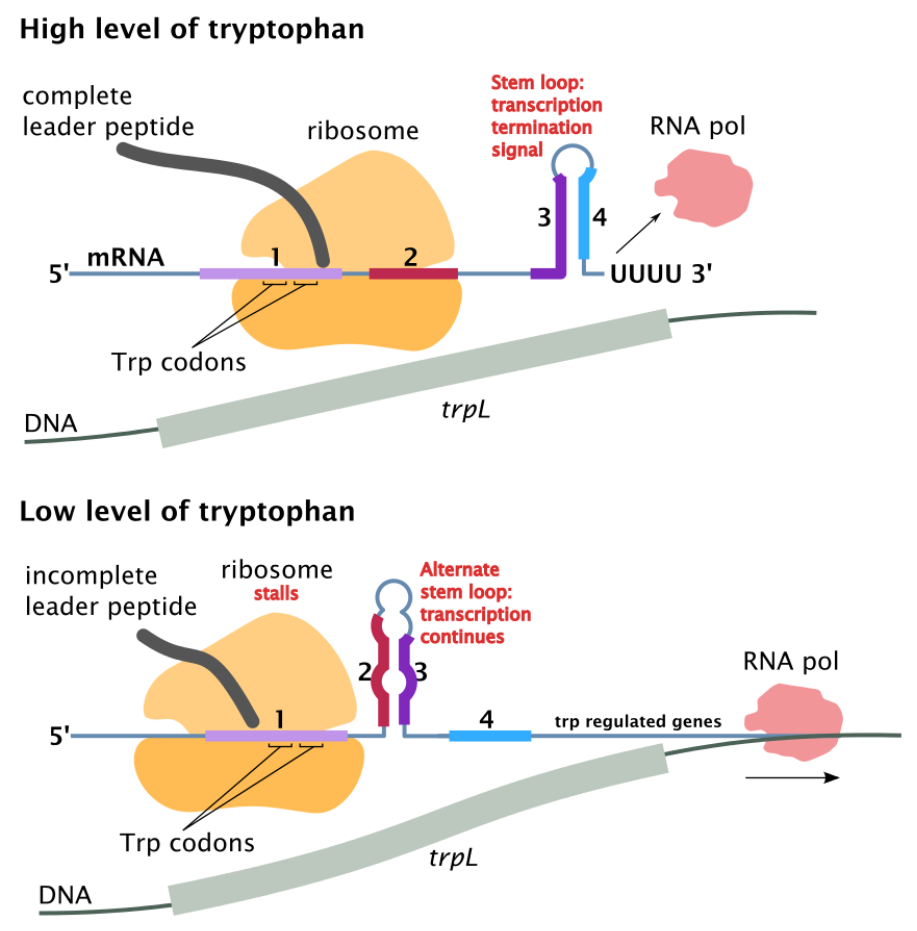
\includegraphics[width = 0.7 \linewidth]{9_tryptophan.png}
    \caption{Аттенюация на примере триптофанового оперона.}
    \label{fig:9_tryptophan}
\end{figure}



\subsection{Промоторы эукариот}

Самое главное отличие эукариотического промотора от прокариотического - \textbf{промотор у каждого гена эукариот свой, оперонов у эукариот нет}.

\subsection{Энхансеры и сайленсеры}
\textbf{Энхансер} (англ. enhancer — усилитель, увеличитель) — небольшой участок ДНК, который после связывания с ним факторов транскрипции стимулирует транскрипцию с основных промоторов гена или группы генов.

\textbf{Сайленсер} - последовательность ДНК, с которой связываются белки-репрессоры транскрипции определенного гена. Связывание белков-репрессоров с сайленсерами приводит к понижению или к полному подавлению синтеза РНК РНК-полимеразой. 

Энхансеры и сайленсеры могут находится на хромосоме (хромосома это комплекс из ДНК и структурных белков гистонов) далеко (даже на другой хромосоме) от промотров генов, транскрипцию которых они регулируют. Тем не менее для их работы необходим физический контакт между ними и промотором. Контакт осуществляется за счёт «выпетливания» ДНК между энхансером/сайленсером и промотором. Молекулярный механизм действия энхансера/сайленсера заключается в том, что он, благодаря собранному на нём белковому комплексу, привлекает/отталкивает РНК-полимеразу II и кофакторы транскрипции в область целевого промотора.

\subsection{Альтернативный сплайсинг}
Между транскрипцией РНК и трансляцией белка у прокариотических клеток ничего не происходит. 

У эукариотических клеток ген состоит из, собственно, участков, кодирующих аминокислоты, составляющие белки, - \textbf{экзонов}, и помойных участков, не кодирующих ничего - \textbf{интронов}. Поэтому после транскрипции гена и до трансляции с него белка у эукариот происходит \textbf{сплайсинг} - вырезание из РНК интронов с оставлением только экзонов.

В результате обычного сплайсинга убираются все интроны, и оставляются все экзоны. А в результате \textbf{альтернативного сплайсинга} получаются самые разные вещи (см. рис. \ref{fig:9_splicing}). Основные вещи, встречающиеся в альтернативном сплайсинге:
\begin{itemize}
    \item пропуск экзона;
    \item удержание интрона (вырезается участок экзона);
    \item взаимоисключающие экзоны (из взаимоисключающих экзонов остается только один);
    \item альтернативный 3'/5' сайт связывания.
\end{itemize}

\begin{figure}[H]
    \centering
    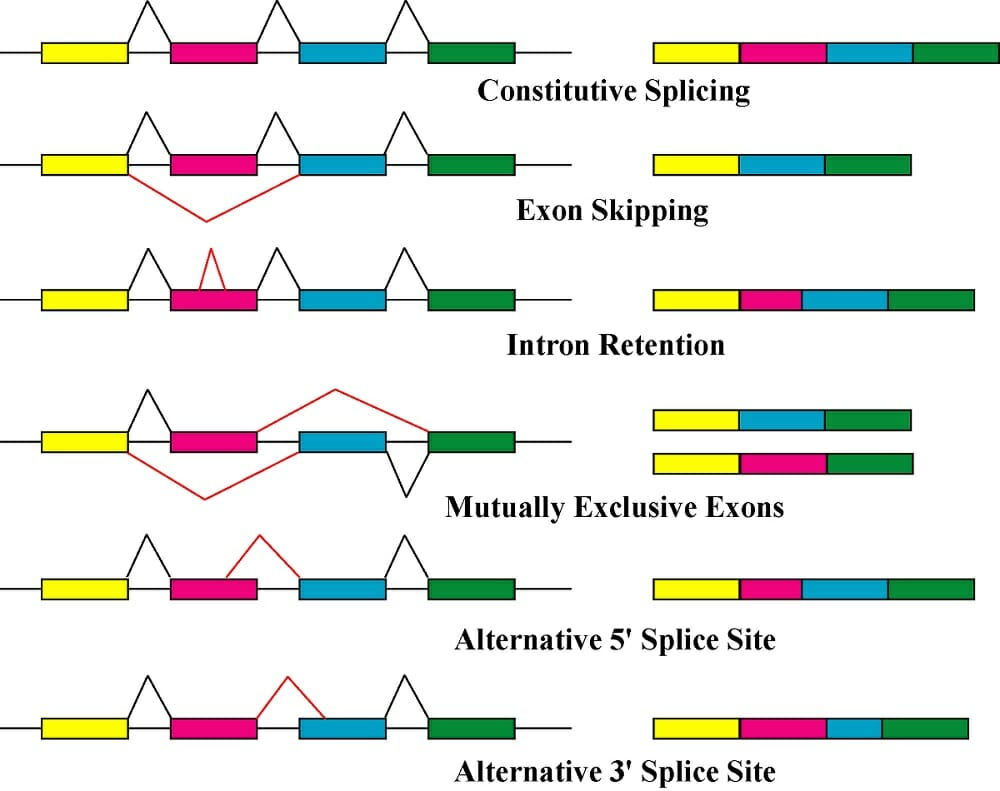
\includegraphics[width = 0.6 \linewidth]{9_splicing.jpg}
    \caption{Вариации альтернативного сплайсинга. В столбце слева мы видим одну и ту же последовательность РНК. Цветные прямоугольники - экзоны, черные линии между ними - интроны. Справа - резьтаты разных процессов альтернативного сплайсинга. В первой строчке обычный сплайсинг.}
    \label{fig:9_splicing}
\end{figure}

	
	\newpage
	
	\section{Репарация ДНК. Эксцизионная репарация NER и BER. Белки эксцизионной репарации (гликозилазы, АП-нуклеазы, UvrABCD, ДНК-полимераза II). SOS-ответ бактерий. Роль генов: recA, lexA, umuCD, uvrABCD}

\subsection{Репарация ДНК}

При репликации происходит большое количество ошибок, их исправлением занимается система репарации. Репарация также помогает при воздействии различных повреждающих агентов, таких как алкилирующие и окисляющие агенты, радиация и прочее. У E.coli известно более 50 генов, контролирующих репарацию, у эукариот их больше. 

Репарация генетических повреждений --- свойство живых организмов восстанавливать нарушения и повреждения, возникшие в ДНК в результате ошибок репликации, а также при воздействии разнообразных эндогенных и экзогенных мутагенных факторов. Важно понимать, что возникающие повреждения --- это не мутации. Мутации --- это наследственное (фиксированное) изменение в нуклеотидной последовательности генома организма.

%Различают следующие механизмы репарации:

%\begin{itemize}
%	\item 
%\end{itemize}

\subsection{Эксцизионная репарация BER}

NER есть Base excision repair или \textbf{Эксцизионная репарация оснований}. Ошибки могут возникать в самом основании. Тогда фермент ДНК-гликозилаза вырезает только азотистое основание от сахарофосфатного остова. Далее AP-эндонуклеаза разрезает сам остов, а ДНК-полимераза и лигаза восстанавливают и сшивают брешь (см. рисунок \ref{fig:10_BER}).

\begin{figure}[H]
	\centering
	\includegraphics[width=0.8\linewidth]{10_BER}
	\caption{Эксцизионная репарация оснований (BER)}
	\label{fig:10_NER}
\end{figure}

\subsection{Эксцизионная репарация NER}

NER есть Nucleotide excision repair или \textbf{Эксцизионная репарация нуклеотидов}. Поврежденный нуклеотид узнается особым комплексом ферментов, вырезается и затем восстанавливается по исходной цепи. Механизм этого типа репарации представлен на рисунке \ref{fig:10_NER}.

\begin{figure}[H]
	\centering
	\includegraphics[width=0.8\linewidth]{10_NER}
	\caption{Эксцизионная репарация нуклеотидов (NER)}
	\label{fig:10_BER}
\end{figure}

\subsection{Белки эксцизионной репарации}

Тут так выходит что если прочитать все подряд, то получится NER у прокариот :)

\subsubsection{Гликозилаза}

Участвует в BER (с нее все начинается), распознает поврежденные основания, неспаренные основания и прочую гадость. После этого разрезает связь азотистого основания с дезоксирибозой, чем удаляет его из ДНК.

\subsubsection{АП-нуклеаза}

Катализирует разрыв внутренних фосфодиэфирных связей в одно-или двунитчатой молекуле ДНК.

\subsubsection{UvrABCD}

Эндонуклаза, образуемая белками UvrA, UvrB и UvrC (вообще все же обычно говорят о UvrABC) и действующей с ней хеликазы UvrD. Сначала UvrA распознает пиримидиновые димеры и прочие крупные повреждения, после чего связывается с UvrB, а дальше прикрепляется UvrC, который вносит надрезы в ДНК по обе стороны от повреждения. После этого хеликаза UvrD расплетает ДНК между насечками, благодаря чему поврежденная цепь высвобождается.

\subsubsection{ДНК-полимераза II}

Участвует в репарации поврежденной ДНК. Обладает способностью 5'-3'-удлинения цепочки и 3'-5'-экзонуклеазным действием и вот понимай как хочешь.

\subsection{SOS-ответ бактерий и роль всевозможных генов}

Сперва вообще скажем, что такое SOS-репарация. Это последняя возможность для ДНК, которая подошла к репликации, имея не устраненные повреждения, сохранить целостность. Если репликация на первом же не устраненном повреждении <<остановится>>, то клетка может погибнуть.  У человека мутации в генах этих белков вызывают наследственное заболевание --- синдром Кокэйна. В процессе эволюции сформировался крайне рискованный механизм репарации, названный <<SOS-репарация ДНК>>. Основная задача такой системы – пройти поврежденный участок ДНК таким образом, чтобы не блокировалось действие ДНК-полимеразы. В результате клетка спасается от гибели на данном этапе и может обеспечить митоз, хотя будут ошибки и высокий риск гибели клетки. Наиболее изучена SOS-репарация у Е.coli, ключевыми белками которой являются белки recA и lexА, поэтому будем смотреть их механизм.

Если в ДНК появляются летальные дефекты, блокирующие ДНК-полимеразу в процессе репликации (например, одноцепочечные разрывы, др.), в клетке активируется система SOS-репарации. Эта система состоит из нескольких десятков белков (recA, lexA, umuD, umuC и др.). В активном состоянии эти белки способствуют формированию полимеразы~V, для которой характерна низкая специфичность (сродство) к материнской цепи ДНК. Это свойство позволяет вставлять в дочернюю цепь нуклеотид, не комплементарный нуклеотиду материнской цепи, преодолевать место повреждения и продолжать процесс репликации. В неповрежденной ДНК активность генов, ответственных за синтез белков полимеразы V, блокируется белком lexA.

Одной из функций белка recA является включение генов umuD и umuC, которые способны замедлять процесс синтеза ДНК при наличии повреждений ДНК. Эти белки могут присоединяться к ДНК-полимеразе~III, снижая ее корректорские функции. Измененный репликационный комплекс продолжает синтез дочерней цепи ДНК на поврежденной матрице, подставляя нуклеотиды случайным образом. В результате дочерние цепи ДНК накапливают ошибки репликации напротив поврежденных нуклеотидов.

\subsubsection{Этапы SOS-репарации}

\begin{enumerate}
	\item В цепи ДНК формируется повреждение, которое ДНК-полимераза~III не может пройти и репликация останавливается. 
	
	\item Активируется синтез белка recA6. Этот белок взаимодействует с белком-репрессором LexA и способствует его аутопротеолизу (расщеплению белка под действием собственных ферментов). После этого и запускается синтез белков, способствующих SOS-репарации. (Начало SOS- ответа определяется взаимодействием белка RecA с белком репрессором LexA. Ответ клетки на повреждающее воздействие начинается с активации протеазной активности белка RecA. Активирующим сигналом может быть присутствие одноцепочечной области в сайте повреждения. Активируясь, RecA-протеаза разрезает белок-репрессор LexA. Белок LexA в неповрежденных клетках функционирует как репрессор многих оперонов, гены которых отвечают за различные репарационные функции. Протеолитическое разрезание репрессора (белка LexA) индуцирует все эти опероны. LexA связывает в своих мишенях так называемый SOS-бокс — участок длиной 20 пар оснований, содержащий консенсус из восьми абсолютно консервативных позиций. Как правило, SOS-бокс входит в состав промотора. LexA репрессирует также ген recA и собственный ген, поэтому в условиях SOS-ответа идёт активный синтез обоих белков. Уровень RecA может повыситься в 50 раз, и в таких концентрациях RecA начинает сам участвовать в эксцизионной репарации. При этом RecA продолжает индуцировать саморасщепление LexA, что не даёт ему функционировать в роли репрессора во время SOS-ответа)
	
	\item Вновьсинтезированный белок RecA закручивается спиралью вокруг одноцепочечной ДНК для ее стабилизации.
	
	\item Активируется синтез белков UmuD, UmuC и прочих.
	
	\item синтезированные белки UmuD и UmuC соединяются со спиралью RecA и образуют комплекс. Основная задача этого комплекса – <<проскочить>> сложный дефект без формирования бреши напротив дефекта. После привлечения комплекса он вытесняет один из структурных компонентов ДНК-полимеразы~III и занимает его место, начиная полимеризацию случайных нуклеотидов на поврежденной матрице. В результате возрастает выживаемость клетки (SOS-репарация) и создаются условия для возникновения мутации (SOS-мутагенез).
	
	\item После прохождения дефектного участка полимераза V отсоединяется от цепи ДНК и работу возобновляет полимераза~III.
\end{enumerate}

Интенсивность SOS-ответа клетки зависит от степени повреждения ДНК, так как только большое количество однонитевой ДНК позволяет активироваться RecA белку в количестве, достаточном для открытия SOS-регулона. Так как белок RecA связывается c LexA в том же сайте, в котором происходит его связывание с двунитевой ДНК, то при запуске SOS-ответа белок RecA не активирует процесс гомологической рекомбинации. В норме при гомологичной рекомбинации SOS-ответ также выражен слабо.

\begin{figure}[H]
	\centering
	\includegraphics[width=0.7\linewidth]{10_gene_functions}
	\caption{Гены и их функции}
\end{figure}

\subsubsection{uvrABCD}

Эндонуклеаза UvrABC представляет собой мультиферментный комплекс в бактериях, участвующих в репарации ДНК путем эксцизионной репарации нуклеотидов, и поэтому ее иногда называют эксинуклеазой. Этот процесс восстановления UvrABC, иногда называемый процессом короткого участка, включает удаление двенадцати нуклеотидов, где произошла генетическая мутация, с последующей ДНК-полимеразой, замена этих аберрантных нуклеотидов правильными нуклеотидами и завершение восстановления ДНК. Субъединицы для этого фермента кодируются в генах uvrA, uvrB и uvrC. Этот ферментный комплекс способен восстанавливать многие виды повреждений, в том числе образование циклобутилдимера.

Как это происходит?

\begin{enumerate}
	\item Два белка UvrA образуют димер, и оба они имеют АТФазную / ГТФазную активность.
	
	\item Димер UvrA связывается с димером UvrB и образует комплекс, способный обнаруживать повреждение ДНК. Димер UvrA функционирует как единица, ответственная за обнаружение повреждения ДНК, вероятно, посредством механизма обнаружения искажений в двойной спирали ДНК.
	
	\item После связывания комплекса UvrA2B2 с предполагаемым поврежденным участком ДНК оборачивается вокруг UvrB.
	
	\item Димер UvrA уходит, и белок UvrC входит и связывается с UvrB и, следовательно, образует новый комплекс UvrBC.
	
	\item UvrC отвечает за расщепление нуклеотидов с обеих сторон повреждения ДНК. Он расщепляет фосфодиэфирную связь на четыре нуклеотида после повреждения ДНК, и расщепляет фосфодиэфирную связь на восемь нуклеотидов выше повреждения ДНК и создает отрезанный из двенадцати нуклеотидов сегмент.
	
	\item Затем вступает ДНК геликаза~II (иногда называемая \textbf{UvrD}) и удаляет вырезанный сегмент, удаляя спаривание оснований. UvrB все еще остается на месте, даже несмотря на то, что UvrC на этом этапе диссоциировал, так как UvrB может быть вовлечен для предотвращения повторного отжига вырезанной ДНК.
	
	\item Входит ДНК-полимераза~I и заполняет правильную нуклеотидную последовательность, отсекая при этом UvrB, и последняя фосфодиэфирная связь завершается с помощью ДНК-лигазы.
\end{enumerate}

	
	\newpage
	
	\section{Классификация белков по функции. Ферменты, классификация ферментов (примеры для основных групп по EC - «Enzyme Commission»/«классификация ферментов»). Хроматографические методы разделения белков: гель-фильтрация, ионообменная хр-я, обращённая фаза, аффинная хр-я.}

\subsection{Функции белков:}

\begin{enumerate}
	\item \textbf{строительная} -- белки участвуют в образовании клеточных и внеклеточных структур (например, белки клеточных мембран);
	
	\item \textbf{транспортная} -- некоторые белки способны присоединять различные вещества и переносить их из одного места клетки в другое (например, \textit{гемоглобин} осуществляет транспорт кислорода);
	
	\item \textbf{регуляционная} -- осуществление регуляции процессов в клетке (например, факторы транскрипции);
	
	\item \textbf{защитная} -- белки имунной защиты (антитела), химической защиты (ферменты печени), физической защиты (\textit{фибриноген} опеспечивает свертываемость крови);
	
	\item \textbf{двигательная} -- сократительные белки актин и миозин обеспечивают сокращение мышц у многоклеточных животных, движений листьев у растений, мерцание ресничек у простейших и т.д.;
	
	\item \textbf{сигнальная} -- в поверхностную мембрану клетки встроены молекулы белков (рецепторы), способных изменять свою третичную структуру в ответ на действие факторов внешней среды, таким образом осуществляя прием сигналов из внешней среды и передачу команд в клетку (например, \textit{адренорецептор} сообщает клетке о присоединении адреналина);
	
	\item \textbf{запасающая} -- казалось бы, клетка питается не белками, но в условиях острого голода, когда ну совсем больше ничего нет, можно и их покушать. У животных и человека при длительном голодании используются белки мышц, эпителиальных тканей и печени. Кажется, \textit{E. coli} умеет кушать свои рибосомы.
	
	\item \textbf{каталитическая} -- или ферментативная (например, \textit{ДНК-полимераза} синтезирует ДНК);
	
	\item \textbf{трофическая} -- близка к транспортной, но не она. Почему-то выделяют в отдельную группу. Основной пример - белок молока (казеин) питает новорожденных. Либо выделяют эту функцию как питание зародышей (например, так делает белок \textit{ихтулин} рыбьей икры).
\end{enumerate}

\subsection{Классификация ферментов:}

\begin{itemize}
	\item \textbf{EC1} -- \textit{оксиредуктаза} -- катализирует перенос электронов, то есть окисление или восстановление. Например, фермент \textit{каталаза} способствует разложению пероксида водорода: \ce{2H2O2 -> 2H2O + O2};
	
	\item \textbf{EC2} -- \textit{трансфераза} -- катализирует перенос функциональных групп и молекулярных остатков от одной молекулы к другой. Например, фермент \textit{гексокиназа} перевешивает фосфат с АТФ на шестой углерод глюкозы:
	\begin{equation*}
	\text{глюкоза + АТФ} \ce{->} \text{глюкозо-6-фосфат + АДФ};
	\end{equation*}
	
	\item \textbf{EC3} -- \textit{гидролаза} -- катализирует гидролиз ковалентной связи. Например, фермент \textit{карбоксипептидаз} гидролизует пептидную связь: 
	\begin{figure}[H]
		\centering
		\includegraphics[width=\linewidth]{Pictures/Hydrolase.jpg}
		\caption{Гидролиз пептидной связи карбоксипептидазой.}
	\end{figure}

	\item \textbf{EC4} -- \textit{лиаза} -- катализирует реакции негидролитического и неокислительного разрыва различных химических связей (разрывает связи, но не присоединяет воду). Например, фермент \textit{метионин-$\gamma$-лиаза} катализирует разложение метионина:
		\begin{figure}[H]
		\centering
		\includegraphics[width=\linewidth]{Pictures/Lease.jpg}
		\caption{Реакция $\gamma$-разложения метионина лиазой.}
	\end{figure}

	\item \textbf{EC5} -- \textit{изомераза} -- катализирует структурные превращения изомеров. Например, фермент \textit{фосфоглюкозоизомераза} делает из глюкозы-6-фосфата фруктозу-6-фосфат:
	\begin{figure}[H]
		\centering
		\includegraphics[width=\linewidth]{Pictures/Izomerase.jpg}
		\caption{Превращение глюкозы с фосфатом во фруктозу с фосфатом (одна из реакций гликолиза).}
	\end{figure}

	\item \textbf{EC6} -- \textit{лигаза} -- катализирует соединение двух молекул с образованием новой химической связи — лигирование. Например, фермент \textit{ДНК-лигаза} способствует образованию фосфодиэфирных связей между 5'- и 3'-концами соседних нуклеотидов в ДНК (важный процесс -- лигирование фрагментов Оказаки при репликации ДНК).
\end{itemize}

\subsection{Хроматографические методы разделения белков}
Смесь растворенных белков пропускают через колонку (полую стеклянную трубку, суженую к низу, как перевернутая бутылка), наполненную маленкими твердыми пористыми шариками. Проходя через такую систему, некоторые белки попадают в поры шариков и задерживаются в них. В зависимости от свойств шариков происходит разделение белков по различным параметрам (см. рисунки!):

\begin{itemize}
	\item \textbf{гель-фильтрация} -- разделение по размеру -- белки маленького размера удершиваются в пористых шариках, а белки большого размера в них не пролезают и просто смываются из колонки;
	
	\item \textbf{ионообменная хроматография} -- разделение по заряду -- наполним колонку заряженными шариками, тогда белки, заряженные противоположно будут притягиваться к шарикам, и чем больше заряд, тем сильнее они удерживаются в колонке;	
	
	\item \textbf{обращённая фаза} -- разделение по гидрофобности/гидрофильности -- интересно, как насыпать в жижу гидрофобных шариков, чтоб они между собой не слиплись? Короче, используется нечто, притягивающее гидрофобные белки. Гидрофильные, ни с чем ни связанные, смываются;
	
	\item \textbf{аффинная хроматография} -- разделение по способности связывать определенный вид молекул -- очевидно, наполнитель из этих самых молекул.
	
	\begin{figure}[H]
	\centering
	\includegraphics[width=\linewidth]{Pictures/Cromato.jpg}
	\caption{Различные виды хроматографии наглядно.}
\end{figure}
\end{itemize}

	
	\newpage
	
	\input{TeX_files/12.tex}	
	
	
	
	
\end{document}